%-----------------------------------------------------------------------------
%
%               Template for sigplanconf LaTeX Class
%
% Name:         sigplanconf-template.tex
%
% Purpose:      A template for sigplanconf.cls, which is a LaTeX 2e class
%               file for SIGPLAN conference proceedings.
%
% Guide:        Refer to "Author's Guide to the ACM SIGPLAN Class,"
%               sigplanconf-guide.pdf
%
% Author:       Paul C. Anagnostopoulos
%               Windfall Software
%               978 371-2316
%               paul@windfall.com
%
% Created:      15 February 2005
%
%-----------------------------------------------------------------------------


\documentclass{llncs}

% The following \documentclass options may be useful:
%
% 10pt          To set in 10-point type instead of 9-point.
% 11pt          To set in 11-point type instead of 9-point.
% authoryear    To obtain author/year citation style instead of numeric.

\usepackage{lmodern}
\usepackage[T1]{fontenc}
\usepackage{xspace}
\usepackage{graphicx}
\usepackage{slatex}
\usepackage{subfig}
\usepackage{upgreek}
\usepackage{varwidth}
\usepackage{verbatim}
\usepackage{color}
\usepackage{stmaryrd}
\usepackage{amsmath}
\usepackage{amssymb}
\usepackage{amsthm}
\usepackage{amscd}
\usepackage{mathtools}

\usepackage{xparse}
\makeatletter
\NewDocumentCommand{\raisedminus}{m}{%
  \raisebox{0.2em}{$\m@th#1{-}$}%
}
\NewDocumentCommand{\unaryminus}{}{%
  \mathbin{%
    \mathchoice{%
      \raisedminus\scriptstyle
    }{%
      \raisedminus\scriptstyle
    }{%
      \raisedminus\scriptscriptstyle
    }{%
      \raisedminus\scriptscriptstyle
    }%
  }%
}
\makeatother

% Hyperref likes to go last
\usepackage[
    bookmarks=true,
    bookmarksnumbered=true,
    breaklinks=false,
    raiselinks=true,
    pdfborder={0 0 0},
    colorlinks=false,
    plainpages=false,
    ]{hyperref}

% This makes hyperlinks point to the tops of figures, not their captions
\usepackage[all]{hypcap}

%%%%%%%%%%%%%%%%%%%%%%%%%%%%%%%%%%%%%%%%%%%%%%%%%%%%%%%%%%%%%%%%%%%%%%%%%%%%%%%%%%%%%%%%%%%%%%%%%%%%%
% BEGIN SPACE HACKS
%%%%%%%%%%%%%%%%%%%%%%%%%%%%%%%%%%%%%%%%%%%%%%%%%%%%%%%%%%%%%%%%%%%%%%%%%%%%%%%%%%%%%%%%%%%%%%%%%%%%%

%\usepackage{showframe}

\makeatletter
\renewcommand\normalsize{%
   \@setfontsize\normalsize\@@ptsize{14.5pt}%
   \abovedisplayskip 8\p@ \@plus2\p@ \@minus2\p@
   \belowdisplayskip \abovedisplayskip
   \abovedisplayshortskip 4\p@ \@plus2\p@ \@minus2\p@
   \belowdisplayshortskip \abovedisplayshortskip
   \renewcommand\arraystretch{0.65}
}

\renewcommand\small{%
   \@setfontsize\small\@ixpt{12pt}%
   \abovedisplayskip 7\p@ \@plus2\p@ \@minus2\p@
   \belowdisplayskip \abovedisplayskip
   %\abovedisplayshortskip 0\p@
   %\belowdisplayshortskip 0\p@
   %\belowdisplayskip \abovedisplayskip
   \renewcommand\arraystretch{0.9}
}

%\setlength\floatsep       {3pt \@minus 1\p@}
%\setlength\textfloatsep   {12pt \@minus 4\p@}
%\setlength\intextsep      {3pt \@minus 1\p@}
%\setlength\dblfloatsep    {3pt \@minus 1\p@}
%\setlength\dbltextfloatsep{3pt \@minus 1\p@}
\makeatother

\usepackage{enumitem}
\setlist{noitemsep,topsep=2pt}
\setitemize{noitemsep,topsep=2pt}
\setenumerate{noitemsep,topsep=2pt}

\newcommand{\smallmathfont}{\small}

%%%%%%%%%%%%%%%%%%%%%%%%%%%%%%%%%%%%%%%%%%%%%%%%%%%%%%%%%%%%%%%%%%%%%%%%%%%%%%%%%%%%%%%%%%%%%%%%%%%%%
% END SPACE HACKS
%%%%%%%%%%%%%%%%%%%%%%%%%%%%%%%%%%%%%%%%%%%%%%%%%%%%%%%%%%%%%%%%%%%%%%%%%%%%%%%%%%%%%%%%%%%%%%%%%%%%%

% Hide subsections in TOC
\setcounter{tocdepth}{1}

\newcounter{maththing}\numberwithin{section}{chapter}

\theoremstyle{definition}
\newtheorem{example}{Example}[chapter]

\theoremstyle{plain}
\newtheorem{definition}[example]{Definition}
\newtheorem{theorem}[example]{Theorem}
\newtheorem{lemma}[example]{Lemma}
\newtheorem{corollary}[example]{Corollary}

\newcommand\numberthis{\addtocounter{equation}{1}\tag{\theequation}}

% puts a little space between the \hrule and captions
\belowcaptionskip 0.25\baselineskip
\newcommand{\bottomhrule}{\vspace{3pt}\hrule\vspace{3pt}}

% keywords
\newcommand{\keyword}[1]{\textbf{#1}}
\newcommand{\mykeyword}[1]{\textbf{\textit{#1}}}

\newcommand\xqed[1]{%
  \leavevmode\unskip\penalty9999 \hbox{}\nobreak\hfill
  \quad\hbox{#1}}

\newcommand{\exampleqed}{\xqed{$\diamondsuit$}}


\newcommand{\lzfclang}{\ensuremath{\lambda_{\text{ZFC}}}\xspace}

%
% Language phase 0: meta
%
% Mostly semantic functions and grammars, definitional extensions to first-order logic

\newcommand{\metadef}{:=}
\newcommand{\metastx}{:\equiv}
\newcommand{\objdef}{:=}
\newcommand{\objstx}{:\equiv}
\newcommand{\gor}{\ |\ }
\newcommand{\meaningof}[1]{\left\llbracket{#1}\right\rrbracket}
\newcommand{\enc}[1]{\mathcal{F}\!\meaningof{#1}}
\newcommand{\stx}[1]{\mathcal{S}\!\meaningof{#1}}
%\newcommand{\metasubst}[3]{{#1}[{#2}:={#3}]}
\newcommand{\metasubst}[3]{s\!\meaningof{{#1},{#2},{#3}}}
\newcommand{\imp}{\Rightarrow}
\newcommand{\rimp}{\Leftarrow}
\DeclareMathOperator{\disjoint}{\mbox{$\not\mspace{-5mu}\i$}}

\renewcommand{\dots}{...}
\newcommand{\setb}[2]{\lbrace {#1} \ \lvert\ {#2} \rbrace}

\newcommand{\justdenom}[1]{\mspace{-4mu} {} \atop {#1} \mspace{-4mu}}
\newcommand{\djustdenom}[1]{\displaystyle{\justdenom{#1}}}


%
% Language phase 1: first-order logic
%

% Common notation and names

\newcommand{\set}[1]{\{{#1}\}}
\newcommand{\seq}[1]{\left({#1}\right)}
\newcommand{\pair}[1]{\langle{#1}\rangle}
\newcommand{\dpair}[1]{\left\langle{#1}\right\rangle}

\newcommand{\band}{\wedge}
\newcommand{\pand}{\big\wedge}
\newcommand{\bor}{\vee}
\newcommand{\por}{\big\vee}

\newcommand{\Bool}{\mathbb{B}}
\newcommand{\Nat}{\mathbb{N}}
\newcommand{\Int}{\mathbb{Z}}
\newcommand{\Rat}{\mathbb{Q}}
\renewcommand{\Re}{\mathbb{R}}
\renewcommand{\P}{\mathbb{P}}

\newcommand{\U}{\textstyle\bigcup}
\renewcommand{\u}{\cup}
\newcommand{\I}{\textstyle\bigcap}
\renewcommand{\i}{\cap}
\newcommand{\wo}{\backslash}
\let\oldemptyset\emptyset
\renewcommand{\emptyset}{\varnothing}
\newcommand{\powerset}{\mathcal{P}}

\newcommand{\Forall}[1]{\forall\,{#1}\ldotp\,}
\newcommand{\Exists}[1]{\exists\,{#1}\ldotp\,}
\newcommand{\ExistsOne}[1]{\exists\char`^\,{#1}\ldotp\,}
\newcommand{\The}[1]{\iota\,{#1}\ldotp\,}

\newcommand{\tto}{\Rightarrow}
%\newcommand{\bijto}{\xrightarrow{\mathrm{bij}}}
\newcommand{\bijto}{\leftrightarrow}
\newcommand{\Ord}{\mathit{Ord}}

\newcommand{\A}{\mathcal{A}}
\newcommand{\B}{\mathcal{B}}
\newcommand{\C}{\mathcal{C}}
\newcommand{\E}{\mathcal{E}}
\newcommand{\V}{\mathcal{V}}

\newcommand{\pnand}{\mathit{nand}}
\newcommand{\w}{\backslash}

% Invented notation and names

\newcommand{\myfun}[1]{\mathit{#1}}
\newcommand{\encset}{\myfun{set}}
\newcommand{\lex}{\myfun{lex}}
\newcommand{\addset}{\myfun{put}}

%\newcommand{\dto}{\Downarrow}
% makes the horizontal spacing around the arrow nice:
\DeclareMathOperator{\dto}{\Downarrow}

\newcommand{\plusomega}{+_\lnat}
\newcommand{\timesomega}{\times_\lnat}

\newcommand{\plusint}{+_Z}
\newcommand{\minusint}{-_Z}
\newcommand{\timesint}{\times_Z}
\newcommand{\equalint}{=_{\mathsf{Z}}}

\newcommand{\plusz}{+_\Int}
\newcommand{\minusz}{-_\Int}
\newcommand{\timesz}{\times_\Int}

\newcommand{\equalrat}{=_{\mathsf{Q}}}
\newcommand{\plusq}{+_\Rat}
\newcommand{\minusq}{-_\Rat}
\newcommand{\timesq}{\times_\Rat}
\newcommand{\divq}{\div_\Rat}

%
% Language phase 2: lambda_ZFC
%

\newcommand{\objlang}[1]{\mathsf{#1}}
%\newcommand{\objlang}[1]{\mathtt{#1}}

\renewcommand{\choose}{\mathcal{E}}
%\newcommand{\Choose}[1]{\choose\,{#1}\ldotp\,}
\newcommand{\Choose}[1]{\set{#1}\ldotp\,}

\newcommand{\domain}{\objlang{domain}}
\newcommand{\range}{\objlang{range}}
\newcommand{\image}{\objlang{image}}
\newcommand{\filter}{\objlang{select}}

\newcommand{\lunion}[1]{{\textstyle\U}\ {#1}}
\newcommand{\lpowerset}[1]{\powerset\ {#1}}
\newcommand{\limage}[2]{{\objlang{image}}\ {#1}\ {#2}}
\newcommand{\lorder}[1]{{\objlang{card}}\ {#1}}
\newcommand{\ltake}[1]{{\objlang{take}}\ {#1}}
\newcommand{\lemptyset}{\oldemptyset}
\newcommand{\lnat}{\upomega}
\newcommand{\lif}[3]{{\objlang{if}}\ {#1}\ {#2}\ {#3}}
\newcommand{\ltrue}{\objlang{true}}
\newcommand{\lfalse}{\objlang{false}}
\newcommand{\lfun}{\lambda\ldotp\,}

\newcommand{\fun}[1]{\lambda\mspace{2mu}{#1}\ldotp\,}

\newcommand{\tvar}{t_\mathrm{var}}
\newcommand{\tapp}{t_\mathrm{app}}
\newcommand{\tif}{t_\mathrm{if}}
\newcommand{\tin}{t_\in}
\newcommand{\tunion}{t_\u}
\newcommand{\ttake}{t_\mathrm{take}}
\newcommand{\tpowerset}{t_\powerset}
\newcommand{\timage}{t_\mathrm{image}}
\newcommand{\torder}{t_\mathrm{card}}
\newcommand{\tset}{t_\mathrm{set}}
\newcommand{\tatom}{t_\mathrm{atom}}
\newcommand{\tfun}{t_\lambda}
\newcommand{\atrue}{a_\mathrm{true}}
\newcommand{\afalse}{a_\mathrm{false}}
\newcommand{\ttrue}{t_\mathrm{true}}
\newcommand{\tfalse}{t_\mathrm{false}}

\newcommand{\Vatom}{V_\mathrm{atom}}
\newcommand{\Vset}{V_\mathrm{set}}
\newcommand{\Vfun}{V_\lambda}
\newcommand{\Evar}{E_\mathrm{var}}
\newcommand{\Eapp}{E_\mathrm{app}}
\newcommand{\Eset}{E_\mathrm{set}}
\newcommand{\Eif}{E_\mathrm{if}}
\newcommand{\Ein}{E_\in}
\newcommand{\Eunion}{E_\u}
\newcommand{\Epowerset}{E_\powerset}
\newcommand{\Eimage}{E_\mathrm{image}}
\newcommand{\Eorder}{E_\mathrm{card}}

\newcommand{\fst}{\myfun{fst}}
\newcommand{\snd}{\myfun{snd}}

\newcommand{\jand}{\;\;\,}

\newenvironment{displaybreaks}%
{%
	\begingroup%
	\allowdisplaybreaks%
}%
{%
	\endgroup%
	\ignorespacesafterend%
}

%\excludecomment{proof}

\newcommand{\figref}[1]{Fig.~\ref{#1}}
\newcommand{\figsref}[1]{Figs.~\ref{#1}}

\newcommand{\arrow}{\rightsquigarrow}

\newcommand{\restrict}[1]{\lvert_{#1}}
\newcommand{\pto}{\rightharpoonup}
\newcommand{\Un}{\mathcal{U}}

\newcommand{\join}{\vee}

\newcommand{\conv}{^{\mspace{-2mu}\Downarrow\mspace{-2mu}}}

\newcommand{\meaningofconv}[1]{\left\llbracket{#1}\right\rrbracket\conv}

\newcommand{\arrowlift}{\ensuremath{lift}}
\newcommand{\arrowarr}{\ensuremath{arr}}
\newcommand{\arrowcomp}{\ensuremath{{>}\mspace{-6mu}{>}\mspace{-6mu}{>}}}
\newcommand{\arrowpair}{\ensuremath{\mathit{\&\mspace{-7.5mu}\&\mspace{-7.5mu}\&}}}
\newcommand{\arrowif}{\ensuremath{ifte}}
\newcommand{\arrowconvif}{\ensuremath{ifte\conv}}
\newcommand{\arrowlazy}{\ensuremath{lazy}}
\newcommand{\arrowapp}{\ensuremath{app}}
\newcommand{\arrowrun}{\ensuremath{run}}
\newcommand{\arrowget}{\ensuremath{get}}
\newcommand{\arrowerror}{\ensuremath{error}}
\newcommand{\arrowtrans}{\ensuremath{\eta}}

\newcommand{\gen}{_\mathrm{a}}
\newcommand{\genb}{_\mathrm{b}}
\newcommand{\genc}{_\mathrm{a^{\mspace{-2mu}*}}}
\newcommand{\gend}{_\mathrm{b^{\mspace{-2mu}*}}}

\DeclareMathOperator{\botto}{\arrow_{\mspace{-3mu}\bot}}
\newcommand{\arrbot}{\arrowarr_{\mspace{-3mu}\bot}}
\newcommand{\compbot}{\arrowcomp_{\mspace{-5mu}\bot}}
\newcommand{\pairbot}{\arrowpair_{\mspace{-3mu}\bot}}
\newcommand{\ifbot}{\arrowif_{\mspace{-2mu}\bot}}
\newcommand{\lazybot}{\arrowlazy_{\mspace{-2mu}\bot}}

\newcommand{\map}{_\mathrm{map}}
\DeclareMathOperator{\mapto}{\arrow_{\mspace{-21mu}\map}}
\newcommand{\liftmap}{\arrowlift\map}
\newcommand{\arrmap}{\arrowarr\map}
\newcommand{\compmap}{\arrowcomp\map}
\newcommand{\pairmap}{\arrowpair\map}
\newcommand{\ifmap}{\arrowif\map}
\newcommand{\lazymap}{\arrowlazy\map}

\newcommand{\pre}{_\mathrm{pre}}
\DeclareMathOperator{\preto}{\arrow_{\mspace{-19mu}\pre}}
\newcommand{\liftpre}{\arrowlift\pre}
\newcommand{\arrpre}{\arrowarr\pre}
\newcommand{\comppre}{\arrowcomp\pre}
\newcommand{\pairpre}{\arrowpair\pre}
\newcommand{\ifpre}{\arrowif\pre}
\newcommand{\lazypre}{\arrowlazy\pre}

\newcommand{\pbot}{{\bot^{\mspace{-4mu}*}}}
\DeclareMathOperator{\pbotto}{\arrow_{\mspace{-3mu}\pbot}}
\newcommand{\arrpbot}{\arrowarr_{\mspace{-3mu}\pbot}}
\newcommand{\comppbot}{\arrowcomp_{\mspace{-5mu}\pbot}}
\newcommand{\pairpbot}{\arrowpair_{\mspace{-3mu}\pbot}}
\newcommand{\ifpbot}{\arrowif_{\mspace{-2mu}\pbot}}
\newcommand{\convifpbot}{\arrowconvif_{\mspace{-2mu}\pbot}}
\newcommand{\lazypbot}{\arrowlazy_{\mspace{-2mu}\pbot}}

\newcommand{\pmap}{_\mathrm{map^{\mspace{-2mu}*}}}
\DeclareMathOperator{\pmapto}{\arrow_{\mspace{-22mu}_{\mathrm{map*}}}}
\newcommand{\liftpmap}{\arrowlift\pmap}
\newcommand{\arrpmap}{\arrowarr\pmap}
\newcommand{\comppmap}{\arrowcomp\pmap}
\newcommand{\pairpmap}{\arrowpair\pmap}
\newcommand{\ifpmap}{\arrowif\pmap}
\newcommand{\convifpmap}{\arrowconvif\pmap}
\newcommand{\lazypmap}{\arrowlazy\pmap}

\newcommand{\ppre}{_\mathrm{pre^{\mspace{-2mu}*}}}
\DeclareMathOperator{\ppreto}{\arrow_{\mspace{-19mu}_{\mathrm{pre*}}}}
\newcommand{\liftppre}{\arrowlift\ppre}
\newcommand{\arrppre}{\arrowarr\ppre}
\newcommand{\compppre}{\arrowcomp\ppre}
\newcommand{\pairppre}{\arrowpair\ppre}
\newcommand{\ifppre}{\arrowif\ppre}
\newcommand{\convifppre}{\arrowconvif\ppre}
\newcommand{\lazyppre}{\arrowlazy\ppre}

\newcommand{\prepto}{\pto_{\mspace{-19mu}\pre}}

\DeclareMathVersion{sans}
\SetSymbolFont{operators}{sans}{T1}{\sfdefault}{m}{n}
\SetSymbolFont{letters}{sans}{T1}{\sfdefault}{m}{n}
\SetMathAlphabet\mathbf{sans}{T1}{\sfdefault}{bx}{n}
\SetMathAlphabet\mathsf{sans}{T1}{\sfdefault}{m}{n}
\SetMathAlphabet\mathit{sans}{T1}{\rmdefault}{m}{it}

\DeclareSymbolFont{greekletters}{OML}{cmss}{m}{n}
\DeclareMathSymbol{\Gamma}  {\mathord}{greekletters}{"00}
\DeclareMathSymbol{\Delta}  {\mathord}{greekletters}{"01}
\DeclareMathSymbol{\Theta}  {\mathord}{greekletters}{"02}
\DeclareMathSymbol{\Lambda} {\mathord}{greekletters}{"03}
\DeclareMathSymbol{\Xi}     {\mathord}{greekletters}{"04}
\DeclareMathSymbol{\Pi}     {\mathord}{greekletters}{"05}
\DeclareMathSymbol{\Sigma}  {\mathord}{greekletters}{"06}
\DeclareMathSymbol{\Upsilon}{\mathord}{greekletters}{"07}
\DeclareMathSymbol{\Phi}    {\mathord}{greekletters}{"08}
\DeclareMathSymbol{\Psi}    {\mathord}{greekletters}{"09}
\DeclareMathSymbol{\Omega}  {\mathord}{greekletters}{"0A}

\DeclareMathSymbol{\alpha}{\mathord}{greekletters}{"0B}
\DeclareMathSymbol{\beta}{\mathord}{greekletters}{"0C}
\DeclareMathSymbol{\gamma}{\mathord}{greekletters}{"0D}
\DeclareMathSymbol{\delta}{\mathord}{greekletters}{"0E}
\DeclareMathSymbol{\epsilon}{\mathord}{greekletters}{"0F}
\DeclareMathSymbol{\zeta}{\mathord}{greekletters}{"10}
\DeclareMathSymbol{\eta}{\mathord}{greekletters}{"11}
\DeclareMathSymbol{\theta}{\mathord}{greekletters}{"12}
\DeclareMathSymbol{\iota}{\mathord}{greekletters}{"13}
\DeclareMathSymbol{\kappa}{\mathord}{greekletters}{"14}
\DeclareMathSymbol{\lambda}{\mathord}{greekletters}{"15}
\DeclareMathSymbol{\mu}{\mathord}{greekletters}{"16}
\DeclareMathSymbol{\nu}{\mathord}{greekletters}{"17}
\DeclareMathSymbol{\xi}{\mathord}{greekletters}{"18}
\DeclareMathSymbol{\pi}{\mathord}{greekletters}{"19}
\DeclareMathSymbol{\rho}{\mathord}{greekletters}{"1A}
\DeclareMathSymbol{\sigma}{\mathord}{greekletters}{"1B}
\DeclareMathSymbol{\tau}{\mathord}{greekletters}{"1C}
\DeclareMathSymbol{\upsilon}{\mathord}{greekletters}{"1D}
\DeclareMathSymbol{\phi}{\mathord}{greekletters}{"1E}
\DeclareMathSymbol{\chi}{\mathord}{greekletters}{"1F}
\DeclareMathSymbol{\psi}{\mathord}{greekletters}{"20}
\DeclareMathSymbol{\omega}{\mathord}{greekletters}{"21}
\DeclareMathSymbol{\varepsilon}{\mathord}{greekletters}{"22}
\DeclareMathSymbol{\vartheta}{\mathord}{greekletters}{"23}
\DeclareMathSymbol{\varpi}{\mathord}{greekletters}{"24}
\DeclareMathSymbol{\varrho}{\mathord}{greekletters}{"25}
\DeclareMathSymbol{\varsigma}{\mathord}{greekletters}{"26}

\DeclareSymbolFont{fixpunct}{T1}{\rmdefault}{m}{n}
\DeclareSymbolFont{fixpunctoml}{OML}{\rmdefault}{m}{n}
\DeclareMathSymbol{,}{\mathpunct}{fixpunct}{`,}
\DeclareMathSymbol{.}{\mathord}{fixpunct}{`.}
\DeclareMathSymbol{\ldotp}{\mathord}{fixpunct}{`.}
\DeclareMathSymbol{!}{\mathord}{letters}{`-}
\DeclareMathSymbol{/}{\mathpunct}{fixpunct}{`/}
\DeclareMathSymbol{\rightharpoonup}{\mathrel}{fixpunctoml}{"2A}
\DeclareMathSymbol{^}{\mathpunct}{fixpunct}{`!}

\DeclareSymbolFont{numbers}{T1}{pvh}{m}{n}
\SetSymbolFont{numbers}{sans}{T1}{\rmdefault}{m}{n}
\DeclareMathSymbol{0}{\mathalpha}{numbers}{"30}
\DeclareMathSymbol{1}{\mathalpha}{numbers}{"31}
\DeclareMathSymbol{2}{\mathalpha}{numbers}{"32}
\DeclareMathSymbol{3}{\mathalpha}{numbers}{"33}
\DeclareMathSymbol{4}{\mathalpha}{numbers}{"34}
\DeclareMathSymbol{5}{\mathalpha}{numbers}{"35}
\DeclareMathSymbol{6}{\mathalpha}{numbers}{"36}
\DeclareMathSymbol{7}{\mathalpha}{numbers}{"37}
\DeclareMathSymbol{8}{\mathalpha}{numbers}{"38}
\DeclareMathSymbol{9}{\mathalpha}{numbers}{"39}

\renewcommand{\notin}{\not\in}

\newcommand\mathtest[2]{\mathchoice{#1}{#2}{#2}{#2}}

\newenvironment{lzfcenv}[1][l]%
{%
	\begin{array}[t]{@{}#1@{}}%
}%
{%
	\end{array}%
}

\newcommand{\tab}{\ \ \ }

\newcommand{\lzfc}[2][l]{\begin{lzfcenv}[#1]#2\end{lzfcenv}}
\newcommand{\tlzfc}[1]{\ensuremath{#1}}

\newcommand{\lzfcsplit}[2][@{}]{\lzfc[r #1 l]{#2}}

\newcommand{\lzfclet}[2]{\lzfc{let\ \ \lzfc[r@{\ \objdef\ }l]{#1} \\ \lzfc{\tab in\ \ #2}}}
\newcommand{\lzfccond}[2][\ \longrightarrow\ ]{\lzfc{cond\ \ \lzfc[l@{\ {#1}\ }l]{#2}}}
\newcommand{\lzfccase}[3][\ \longrightarrow\ ]{\lzfc{case\ \ {#2}\\\ \ \lzfc[l@{\ {#1}\ }l]{#3}}}

\newcommand{\dash}{\text{-}}

%
% Racket syntax (must be last - or at least \defschememathescape must be - see last line)
%

% DrRacket's default colors
\definecolor{identifiercolor}{rgb}{0.15,0.15,0.5}
\definecolor{keywordcolor}{rgb}{0.0,0.0,0.0}
\definecolor{constantcolor}{rgb}{0.16,0.5,0.15}
\definecolor{parenthesiscolor}{rgb}{0.52,0.24,0.14}

\def\keywordfont#1{\textcolor{keywordcolor}{#1}}
\def\variablefont#1{\textcolor{identifiercolor}{#1}}
\def\constantfont#1{\textcolor{constantcolor}{#1}}
\def\datafont#1{\textcolor{parenthesiscolor}{#1}}

\makeatletter
\def\mycodehook{\tt\color{parenthesiscolor}\@setfontsize\small{10pt}{11pt minus0.5pt}}
\makeatother
\let\schemecodehook\mycodehook
\setlength{\leftcodeskip}{\parindent}

\setlength{\leftcodeskip}{0pt}
\setlength{\rightcodeskip}{0pt plus 1fil}
\setlength{\abovecodeskip}{0.5\abovedisplayskip}
\setlength{\belowcodeskip}{0.5\belowdisplayskip}

\unsetspecialsymbol{.}
\unsetspecialsymbol{...}
\unsetspecialsymbol{-}
\unsetspecialsymbol{1-}
\unsetspecialsymbol{-1+}

\setspecialsymbol{<blank-line>}{\va{}}
\setspecialsymbol{lambda}{\va{$\mathtt{\lambda}$}}
\setspecialsymbol{λ}{\va{$\mathtt{\lambda}$}}
\setspecialsymbol{~}{\va{$\mathtt{\sim}$}}
\setspecialsymbol{_}{\va{$\underbar{ }$}}
\setspecialsymbol{Omega}{\va{$\mathtt{\Omega}$}}
\setspecialsymbol{omega}{\va{$\mathtt{\omega}$}}
\setspecialsymbol{Ω}{\va{$\mathtt{\Omega}$}}
\setspecialsymbol{ω}{\va{$\mathtt{\omega}$}}

\setkeyword{define/drbayes struct/drbayes}

\defschememathescape{$}



\begin{comment}
Does the phrase "operational lambda-calculus" make sense? I intend to mean that it has an operational semantics, or is intended to ...
\end{comment}


\newsavebox{\codebox}

\renewcommand{\paragraph}[1]{\vspace{0.5\baselineskip}\noindent\textbf{{#1}.}\hspace{0.25\baselineskip}}
\newcommand{\smallmathfont}{\fontsize{7.5}{9}\selectfont}

\newenvironment{displaybreaks}%
{%
	\begingroup%
	\allowdisplaybreaks%
}%
{%
	\endgroup%
	\ignorespacesafterend%
}

\excludecomment{proof}

\newcommand{\figref}[1]{Fig.~\ref{#1}}
\newcommand{\figsref}[1]{Figs.~\ref{#1}}

\newcommand{\arrow}{\rightsquigarrow}

\newcommand{\restrict}[1]{\lvert_{#1}}
\newcommand{\pto}{\rightharpoonup}
\newcommand{\Univ}{\mathbb{U}}
\newcommand{\Un}{\mathcal{U}}

\newcommand{\join}{\vee}

\newcommand{\conv}{^{\mspace{-2mu}\Downarrow\mspace{-2mu}}}

\newcommand{\meaningofconv}[1]{\left\llbracket{#1}\right\rrbracket\conv}

\newcommand{\arrowlift}{\ensuremath{lift}}
\newcommand{\arrowarr}{\ensuremath{arr}}
\newcommand{\arrowcomp}{\ensuremath{{>}\mspace{-6mu}{>}\mspace{-6mu}{>}}}
\newcommand{\arrowpair}{\ensuremath{\mathit{\&\mspace{-7.5mu}\&\mspace{-7.5mu}\&}}}
\newcommand{\arrowif}{\ensuremath{ifte}}
\newcommand{\arrowconvif}{\ensuremath{ifte\conv}}
\newcommand{\arrowlazy}{\ensuremath{lazy}}
\newcommand{\arrowapp}{\ensuremath{app}}
\newcommand{\arrowrun}{\ensuremath{run}}
\newcommand{\arrowget}{\ensuremath{get}}
\newcommand{\arrowerror}{\ensuremath{error}}
\newcommand{\arrowtrans}{\ensuremath{\eta}}

\newcommand{\gen}{_\mathrm{a}}
\newcommand{\genb}{_\mathrm{b}}
\newcommand{\genc}{_\mathrm{a^{\mspace{-2mu}*}}}
\newcommand{\gend}{_\mathrm{b^{\mspace{-2mu}*}}}

\DeclareMathOperator{\botto}{\arrow_{\mspace{-3mu}\bot}}
\newcommand{\arrbot}{\arrowarr_{\mspace{-3mu}\bot}}
\newcommand{\compbot}{\arrowcomp_{\mspace{-5mu}\bot}}
\newcommand{\pairbot}{\arrowpair_{\mspace{-3mu}\bot}}
\newcommand{\ifbot}{\arrowif_{\mspace{-2mu}\bot}}
\newcommand{\lazybot}{\arrowlazy_{\mspace{-2mu}\bot}}

\newcommand{\map}{_\mathrm{map}}
\DeclareMathOperator{\mapto}{\arrow_{\mspace{-21mu}\map}}
\newcommand{\liftmap}{\arrowlift\map}
\newcommand{\arrmap}{\arrowarr\map}
\newcommand{\compmap}{\arrowcomp\map}
\newcommand{\pairmap}{\arrowpair\map}
\newcommand{\ifmap}{\arrowif\map}
\newcommand{\lazymap}{\arrowlazy\map}

\newcommand{\pre}{_\mathrm{pre}}
\DeclareMathOperator{\preto}{\arrow_{\mspace{-19mu}\pre}}
\newcommand{\liftpre}{\arrowlift\pre}
\newcommand{\arrpre}{\arrowarr\pre}
\newcommand{\comppre}{\arrowcomp\pre}
\newcommand{\pairpre}{\arrowpair\pre}
\newcommand{\ifpre}{\arrowif\pre}
\newcommand{\lazypre}{\arrowlazy\pre}

\newcommand{\pbot}{{\bot^{\mspace{-4mu}*}}}
\DeclareMathOperator{\pbotto}{\arrow_{\mspace{-3mu}\pbot}}
\newcommand{\arrpbot}{\arrowarr_{\mspace{-3mu}\pbot}}
\newcommand{\comppbot}{\arrowcomp_{\mspace{-5mu}\pbot}}
\newcommand{\pairpbot}{\arrowpair_{\mspace{-3mu}\pbot}}
\newcommand{\ifpbot}{\arrowif_{\mspace{-2mu}\pbot}}
\newcommand{\convifpbot}{\arrowconvif_{\mspace{-2mu}\pbot}}
\newcommand{\lazypbot}{\arrowlazy_{\mspace{-2mu}\pbot}}

\newcommand{\pmap}{_\mathrm{map^{\mspace{-2mu}*}}}
\DeclareMathOperator{\pmapto}{\arrow_{\mspace{-22mu}_{\mathrm{map*}}}}
\newcommand{\liftpmap}{\arrowlift\pmap}
\newcommand{\arrpmap}{\arrowarr\pmap}
\newcommand{\comppmap}{\arrowcomp\pmap}
\newcommand{\pairpmap}{\arrowpair\pmap}
\newcommand{\ifpmap}{\arrowif\pmap}
\newcommand{\convifpmap}{\arrowconvif\pmap}
\newcommand{\lazypmap}{\arrowlazy\pmap}

\newcommand{\ppre}{_\mathrm{pre^{\mspace{-2mu}*}}}
\DeclareMathOperator{\ppreto}{\arrow_{\mspace{-19mu}_{\mathrm{pre*}}}}
\newcommand{\liftppre}{\arrowlift\ppre}
\newcommand{\arrppre}{\arrowarr\ppre}
\newcommand{\compppre}{\arrowcomp\ppre}
\newcommand{\pairppre}{\arrowpair\ppre}
\newcommand{\ifppre}{\arrowif\ppre}
\newcommand{\convifppre}{\arrowconvif\ppre}
\newcommand{\lazyppre}{\arrowlazy\ppre}

\newcommand{\prepto}{\pto_{\mspace{-19mu}\pre}}

\title{Running Probabilistic Programs Backward}

\author{Neil Toronto and Jay McCarthy\\
\footnotesize{\texttt{neil.toronto@gmail.com} and \texttt{jay@cs.byu.edu}}}
\institute{PLT @ Brigham Young University, Provo, Utah, USA}

\date{}

\begin{document}

\maketitle

\begin{abstract}
To be useful in Bayesian practice, a probabilistic language must support conditioning: imposing constraints in a way that preserves the relative probabilities of program outputs.
Every language to date that supports probabilistic conditioning also places seemingly artificial restrictions on legal programs, such as disallowing recursion and restricting conditions to simple equality constraints such as $x = \mathrm{2}$.

We develop a semantics for a first-order language with recursion, probabilistic choice and conditioning.
Distributions over program outputs are defined by the probabilities of their preimages, a measure-theoretic approach that ensures the language is not artificially limited.

Preimages are generally uncomputable, so we derive an approximating semantics for computing rectangular covers of preimages.
We implement the approximating semantics in Haskell and Typed Racket, and demonstrate its expressive power using stochastic ray tracing.
\end{abstract}

\keywords Probability, Semantics, Domain-Specific Languages

%%%%%%%%%%%%%%%%%%%%%%%%%%%%%%%%%%%%%%%%%%%%%%%%%%%%%%%%%%%%%%%%%%%%%%%%%%%%%%%%%%%%%%%%%%%%%%%%%%%%%
%%%%%%%%%%%%%%%%%%%%%%%%%%%%%%%%%%%%%%%%%%%%%%%%%%%%%%%%%%%%%%%%%%%%%%%%%%%%%%%%%%%%%%%%%%%%%%%%%%%%%
%%%%%%%%%%%%%%%%%%%%%%%%%%%%%%%%%%%%%%%%%%%%%%%%%%%%%%%%%%%%%%%%%%%%%%%%%%%%%%%%%%%%%%%%%%%%%%%%%%%%%

\section{Introduction}

It is primarily Bayesian practice that drives probabilistic language development.
To be useful, a probabilistic language must support \keyword{conditioning}, or imposing constraints in a way that preserves the relative probabilities of outputs.

Unfortunately, there is currently no efficient probabilistic language implementation that supports conditioning and does not restrict legal programs.
Most commonly, languages that support conditioning disallow recursion, allow only discrete or continuous distributions, and restrict conditions to the form $\mathit{x} = \mathit{c}$.

These common language restrictions arise from reasoning about probability using \keyword{densities}, which are functions from random values to \emph{changes} in probability.
While simple and convenient, densities have many limitations.
For example, densities for random values with different dimension are incomparable, and they cannot be defined on infinite products.
Either limitation rules out recursion.

\mathversion{sans}
Densities generally cannot define distributions for the outputs of discontinuous functions.
For example, suppose we want to model a thermometer that reports in the range $[0,100]$, and that the temperature it would report (if it could) is distributed according to a bell curve.
We might encode the process as
\begin{equation}
	t'\ :=\ \lzfclet{t & normal~\mu~1}{max~0~(min~100~t)}
\label{eqn:thermometer-example}
\end{equation}
While $t$'s distribution has a density, the distribution of $t'$ does not.
\mathversion{normal}

Densities disallow all but the simplest conditions.
\keyword{Bayes' law for densities} gives the density of $x$ given an observed $y$ in terms of other densities:
\begin{equation}
	p_x(x\,|\,y)\ =\ \frac{p_y(y\,|\,x) \cdot \pi_x(x)}{\int p_y(y\,|\,x) \cdot \pi_x(x)~dx}
\label{eqn:bayes-law-densities}
\end{equation}
Bayesians interpret probabilistic processes as defining $p_y$ and $\pi_x$, and use~\eqref{eqn:bayes-law-densities} to find the distribution of ``$x$ given $y = c$.''
Even though ``$x$ given $x + y = \mathrm{0}$'' has perfectly sensible distribution, Bayes' law for densities cannot express it.

%\subsection{Probability Measures}

Measure-theoretic probability~\cite{cit:klenke-2006-probability} is widely believed to be able to define every reasonable distribution that densities cannot.
It mainly does this by \emph{assigning probabilities to sets} instead of \emph{assigning changes in probability to values}.
Functions that do so are called \keyword{probability measures}.

If a probability measure $P$ assigns probabilities to subsets of $X$ and $f : X \to Y$, then \keyword{preimage measure} defines the distribution over subsets of $Y$:
\begin{equation}
	\Pr[B] \ = \ P(f^{-1}(B))
\end{equation}
The preimage $f^{-1}(B) = \setb{a \in X}{f(a) \in B}$ is the subset of $X$ for which $f$ yields a value in $B$.
Preimages under $f$ are well-defined regardless of discontinuities.

Measure-theoretic probability supports any kind of condition.
If $\Pr[B] > \mathrm{0}$, the probability of $B' \subseteq Y$ given $B \subseteq Y$ is
$\Pr[B'\,|\,B] = \Pr[B' \i B]\ /\ \Pr[B]$.
%\begin{equation}
%	\Pr[B'\,|\,B]\ =\ \Pr[B' \i B]\ /\ \Pr[B]
%\label{eqn:bayes-law-preimage}
%\end{equation}
If $\Pr[B] = \mathrm{0}$, conditional probabilities can be calculated as the limit of $\Pr[B'\,|\,B_n]$ for positive-probability $B_1 \supseteq B_2 \supseteq B_3 \supseteq \cdots$ whose intersection is $B$.
For example, if $Y = \Re \times \Re$, the distribution of ``$\pair{x,y} \in Y$ given $x + y = \mathrm{0}$'' can be calculated using the descending sequence $B_n = \setb{\pair{x,y} \in Y}{|x + y| < \mathrm{2}^{-n}}$.

Only special families of \keyword{measurable} sets can be assigned probabilities.
Proving measurability, taking limits, and other complications tend to make measure-theoretic probability less attractive, even though it is strictly more powerful.

\subsection{Measure-Theoretic Semantics}

Most purely functional languages allow only nontermination as a side effect, and not probabilistic choice.
Programmers therefore encode probabilistic programs as functions from random sources to outputs.
Monads and other categorical classes such as idioms (i.e. applicative functors) can make doing so easier~\cite{cit:hurd-2002thesis,cit:toronto-2010ifl-bayes}.

It seems this approach should make it easy to interpret probabilistic programs measure-theoretically.
For a probabilistic program $f : X \to Y$, the probability measure on output sets $B \subseteq Y$ should be defined by preimages of $B$ under $f$ and the probability measure on $X$.
Unfortunately, it is difficult to turn this simple-sounding idea into a compositional semantics, for the following reasons.
\begin{enumerate}
	\item Preimages can be defined only for functions with observable domains, which excludes lambdas.%
\label{problem:observable-domain}
	\item If subsets of $X$ and $Y$ must be measurable, taking preimages under $f$ must preserve measurability (we say $f$ itself is measurable). Proving the conditions under which this is true is difficult, especially if $f$ may not terminate.%
\label{problem:measurability}
	\item It is very difficult to define probability measures for arbitrary spaces of measurable functions~\cite{cit:aumann-1961ijm-borel}.%
\label{problem:higher-orderness}
\end{enumerate}
Implementing a language based on such a semantics is complicated because
\begin{enumerate}
	\setcounter{enumi}{3}
	\item Contemporary mathematics is unlike any implementation's host language.%
\label{problem:different-language}
	\item It requires running Turing-equivalent programs backward, efficiently, on possibly uncountable sets of outputs.%
\label{problem:backward-efficient}
\end{enumerate}

We address~\ref{problem:observable-domain} and~\ref{problem:different-language} by developing our semantics in \lzfclang~\cite{cit:toronto-2012flops-lzfc}, a $\lambda$-calculus with infinite sets, and both extensional and intensional functions.
We address~\ref{problem:backward-efficient} by deriving and implementing a \emph{conservative approximation} of the semantics.

We have addressed difficulty~\ref{problem:measurability} by proving that all programs' interpretations as functions are measurable if language primitives are measurable, including uncomputable primitives such as limits and real equality, regardless of nontermination.
The proof interprets programs as extensional functions and applies well-known theorems from measure theory.
The required machinery does not fit in this report; see the full version~\cite{cit:toronto-2014esop-long} for the entire development.

For difficulty~\ref{problem:higher-orderness}, we have discovered that the ``first-orderness'' of arrows~\cite{cit:hughes-2000scp-arrows} is a perfect fit for the ``first-orderness'' of measure theory.

%%%%%%%%%%%%%%%%%%%%%%%%%%%%%%%%%%%%%%%%%%%%%%%%%%%%%%%%%%%%%%%%%%%%%%%%%%%%%%%
%%%%%%%%%%%%%%%%%%%%%%%%%%%%%%%%%%%%%%%%%%%%%%%%%%%%%%%%%%%%%%%%%%%%%%%%%%%%%%%
%%%%%%%%%%%%%%%%%%%%%%%%%%%%%%%%%%%%%%%%%%%%%%%%%%%%%%%%%%%%%%%%%%%%%%%%%%%%%%%
\mathversion{sans}
%%%%%%%%%%%%%%%%%%%%%%%%%%%%%%%%%%%%%%%%%%%%%%%%%%%%%%%%%%%%%%%%%%%%%%%%%%%%%%%
%%%%%%%%%%%%%%%%%%%%%%%%%%%%%%%%%%%%%%%%%%%%%%%%%%%%%%%%%%%%%%%%%%%%%%%%%%%%%%%
%%%%%%%%%%%%%%%%%%%%%%%%%%%%%%%%%%%%%%%%%%%%%%%%%%%%%%%%%%%%%%%%%%%%%%%%%%%%%%%

\subsection{Arrow Solution Overview}

\newcommand{\youarehere}[1]%
{%
\begin{equation}%
\begin{CD}%
X \botto Y   @>\liftpre>>   X \preto Y \\%
@V{\eta_\pbot}VV              @VV{\eta\ppre}V\\%
X \pbotto Y  @>>\liftppre>  X \ppreto Y%
\end{CD}%
\label{#1}%
\end{equation}%
}

We define \emph{exact} and \emph{approximating} semantics.
The exact semantics includes
\begin{itemize}
	\item A semantic function which, like the arrow calculus semantic function~\cite{cit:lindley-2010jfp-arrow-calculus}, transforms first-order programs into the computations of an arbitrary arrow.
	\item Arrows for evaluating expressions in different ways.
\end{itemize}
This commutative diagram describes the relationships among the exact arrows:
\youarehere{eqn:roadmap-diagram1}
In the top row, $X \botto Y$ arrow computations are functions that may raise errors and $X \preto Y$ instances compute preimages.
The computations of the arrows in the bottom row are like those in the top, except they thread an infinite store of random values, and can be constructed to always terminate.
Most of our correctness theorems rely on proofs that every morphism in~\eqref{eqn:roadmap-diagram1} is a homomorphism.

The approximating semantics has the same semantic function, but its arrows $X \preto' Y$ and $X \ppreto' Y$ compute conservative approximations.
Given a library for representing and operating on rectangular sets, it is directly implementable.

%%%%%%%%%%%%%%%%%%%%%%%%%%%%%%%%%%%%%%%%%%%%%%%%%%%%%%%%%%%%%%%%%%%%%%%%%%%%%%%%%%%%%%%%%%%%%%%%%%%%%
%%%%%%%%%%%%%%%%%%%%%%%%%%%%%%%%%%%%%%%%%%%%%%%%%%%%%%%%%%%%%%%%%%%%%%%%%%%%%%%%%%%%%%%%%%%%%%%%%%%%%
%%%%%%%%%%%%%%%%%%%%%%%%%%%%%%%%%%%%%%%%%%%%%%%%%%%%%%%%%%%%%%%%%%%%%%%%%%%%%%%%%%%%%%%%%%%%%%%%%%%%%

\subsection{Operational Metalanguage}

We write programs in \lzfclang~\cite{cit:toronto-2012flops-lzfc}, an untyped, call-by-value, operational $\lambda$-calculus designed for deriving implementable programs from contemporary mathematics.

Many mathematical areas are agnostic to their foundations, but measure theory is developed explicitly in \keyword{ZFC}: Zermelo-Fraenkel set theory with Choice.
ZFC's intensional functions are first-order and it has no general recursion, which makes implementing a language defined by a transformation into ZFC difficult.
%The problem is exacerbated if implementing the language requires approximation.
Targeting \lzfclang instead allows creating an exact semantics and deriving an approximating semantics without changing languages.

In \lzfclang, essentially every set is a value, as well as every lambda and every set of lambdas.
All operations, including operations on infinite sets, are assumed to complete instantly if they terminate.
Almost everything definable in ZFC can be defined by a finite \lzfclang program, and essentially every ZFC theorem applies to \lzfclang's set values without alteration.
Proofs about \lzfclang's set values apply directly to ZFC sets, assuming the existence of an inaccessible cardinal.\footnote{A modest assumption, as ZFC+$\kappa$ is a smaller theory than Coq's~\cite{cit:barras-2010-sets-coq}.}

In \lzfclang, algebraic data structures are encoded as sets; e.g. the pair $\pair{x,y}$ can be encoded as $\set{\set{x},\set{x,y}}$.
Only the \emph{existence} of encodings into sets is important, as it means data structures inherit a defining characteristic of sets: strictness.
More precisely, the lengths of paths to data structure leaves is unbounded, but each path must be finite.
Less precisely, data may be ``infinitely wide'' (such as $\Re$) but not ``infinitely tall'' (such as infinite trees and lists).

%We assume data structures, including pairs, are encoded as \emph{primitive} ordered pairs with the first element a unique tag, so they can be distinguished by checking tags.
%sAccessors such as $fst$ and $snd$ are trivial to define.

Though \lzfclang is untyped, it helps in this work to define an auxiliary type system.
It is manually checked, polymorphic, and characterized by these rules:
\begin{itemize}
	\item A free type variable is universally quantified; if uppercase, it denotes a set.
	\item A set denotes a member of that set.
	\item $x \tto y$ denotes a partial function.
	\item $\pair{x,y}$ denotes a pair of values with types $x$ and $y$.
	\item $Set~x$ denotes a set with members of type $x$.
\end{itemize}
Because the type $Set~X$ denotes the same values as the set $\powerset~X$ (i.e. subsets of the set $X$) we regard them as equivalent.
Similarly, $\pair{X,Y}$ is equivalent to $X \times Y$.

Examples of types are those of the \lzfclang primitives membership $(\in) : x \tto Set~x \tto Bool$, powerset $\powerset : Set~x \tto Set~(Set~x)$, big union $\U : Set~(Set~x) \tto Set~x$, and the \texttt{map}-like $image : (x \tto y) \tto Set~x \tto Set~y$.

We use heavily sugared syntax, with automatic currying, binding forms such as indexed unions $\U_{\mathit{x} \in \mathit{e_A}}\mathit{e}$, destructuring binds as in $swap~\pair{x,y} := \pair{y,x}$, and comprehensions like $\setb{x \in A}{x \in B}$.
We assume logical operators, bounded quantifiers, and typical set operations are defined.

In set theory, extensional functions are encoded as sets of input-output pairs; e.g. 
the increment function for the natural numbers is $\set{\pair{0,1},\pair{1,2},\pair{2,3},...}$.
We call these \keyword{mappings} and intensional functions \keyword{lambdas}, and use \keyword{function} to mean either.
As with lambdas, we use adjacency (e.g. $(f~x)$) to apply mappings.

The set $J \to X$ contains all the total mappings from $J$ to $X$; equivalently, all the vectors of $X$ indexed by $J$ (which may be infinite).
The function
\begin{equation}
\begin{aligned}
	&\pi : J \tto (J \to X) \tto X \\
	&\pi~j~f \ := \ f~j
\end{aligned}
\end{equation}
produces projections. This is particularly useful when $f$ is unnamed.

Any \lzfclang term $\mathit{e}$ used as a truth statement means ``$\mathit{e}$ reduces to $true$.''
Therefore, the terms $(\fun{a}{a})~1$ and $1$ are (externally) unequal, but $(\fun{a}{a})~1 = 1$.

Because of the way \lzfclang's lambda terms are defined, lambda equality is alpha equivalence.
For example, $(\fun{a}{a}) = (\fun{b}{b})$, but not $(\fun{a}{2}) = (\fun{a}{1+1})$.

If $\mathit{e}_1 = \mathit{e}_2$, then $\mathit{e}_1$ and $\mathit{e}_2$ both terminate, and substituting one for the other in an expression does not change its value.
Substitution is also safe if both $\mathit{e}_1$ and $\mathit{e}_2$ do not terminate, leading to a coarser notion of equivalence.

\begin{definition}[observational equivalence]
For terms $\mathit{e_1}$ and $\mathit{e_2}$, $\mathit{e_1} \equiv \mathit{e_2}$ when $\mathit{e_1} = \mathit{e_2}$, or both $\mathit{e_1}$ and $\mathit{e_2}$ do not terminate.
\end{definition}

It might seem helpful to define basic equivalence even more coarsely.
However, we want internal equality and external equivalence to be similar, and we want to be able to extend ``$\equiv$'' with type-specific rules.

We elide proofs to save space.
They are in the full version of this paper~\cite{cit:toronto-2014esop-long}.


%%%%%%%%%%%%%%%%%%%%%%%%%%%%%%%%%%%%%%%%%%%%%%%%%%%%%%%%%%%%%%%%%%%%%%%%%%%%%%%%%%%%%%%%%%%%%%%%%%%%%
%%%%%%%%%%%%%%%%%%%%%%%%%%%%%%%%%%%%%%%%%%%%%%%%%%%%%%%%%%%%%%%%%%%%%%%%%%%%%%%%%%%%%%%%%%%%%%%%%%%%%
%%%%%%%%%%%%%%%%%%%%%%%%%%%%%%%%%%%%%%%%%%%%%%%%%%%%%%%%%%%%%%%%%%%%%%%%%%%%%%%%%%%%%%%%%%%%%%%%%%%%%

\section{Arrows and First-Order Semantics}

Like monads~\cite{cit:wadler-2001-monads} and idioms~\cite{cit:mcbride-2008jfp-idiom}, arrows~\cite{cit:hughes-2000scp-arrows} thread effects through computations in a way that imposes structure.
But arrow computations are always
\begin{itemize}
	\item Function-like: An arrow computation of type $x \arrow y$ must behave like a corresponding function of type $x \tto y$ (in a sense we explain shortly).
	\item First-order: There is no way to derive a computation $app : \pair{x \arrow y, x} \arrow y$ from an arrow's minimal definition.
\end{itemize}
The first property makes arrows a good fit for a compositional translation from expressions to pure functions that operate on random sources.
The second property makes arrows a good fit for a measure-theoretic semantics in particular, as $app$'s corresponding function is generally not measurable~\cite{cit:aumann-1961ijm-borel}.
%Targeting arrows in the semantics therefore gives some assurance that we can meet measure theory's requirement that preimage measure be defined only for measurable functions.

\subsection{Alternative Arrow Definitions and Laws}
\label{sec:arrow-definitions}

To make applying measure-theoretic theorems easier, and to simplify interpreting let-calculus expressions as arrow computations, we do not give typical minimal arrow definitions.
For each arrow $a$, instead of $first\gen$, we define $(\arrowpair\gen)$.
This combinator is typically called \keyword{fanout}, but its use will be clearer if we call it \keyword{pairing}.
One way to strengthen an arrow $a$ is to define an additional combinator $left\gen$, which can be used to choose an arrow computation based on the result of another.
Again, we define a different combinator, $\arrowif\gen$ (``if-then-else'').

In a nonstrict $\lambda$-calculus, defining a choice combinator allows writing recursive functions using nothing but arrow combinators and lifted, pure functions.
However, a strict $\lambda$-calculus needs an extra combinator $\arrowlazy$ for deferring conditional branches.
For example, define the \keyword{function arrow} with choice:
\begin{equation}
\begin{aligned}
	\begin{aligned}[t]
		\arrowarr~f &\ := \ f \\
		(f_1~\arrowcomp~f_2)~a &\ := \ f_2~(f_1~a) \\
		(f_1~\arrowpair~f_2)~a &\ := \ \pair{f_1~a,f_2,a} \\
	\end{aligned}
&\tab\tab
	\begin{aligned}[t]
		\arrowif~f_1~f_2~f_3~a &\ := \ if~(f_1~a)~(f_2~a)~(f_3~a) \\
		\arrowlazy~f~a &\ :=\ f~0~a
	\end{aligned}
\end{aligned}
\label{eqn:function-arrow}
\end{equation}
and try to define the following recursive function:
\begin{equation}
	halt!on!true \ := \ \arrowif~(\arrowarr~id)~(\arrowarr~id)~halt!on!true
\end{equation}
In a strict $\lambda$-calculus, the defining expression does not terminate.
But if the ``else'' branch is $\arrowlazy~\fun{0}{halt!on!true}$, it loops only when applied to $false$.

All of our arrows are arrows with choice, so we simply call them arrows.

\begin{definition}[arrow]Let $1 := \set{0}$. A binary type constructor $(\arrow\gen)$ and
\begin{displaybreaks}
\begin{equation}
\begin{aligned}
	\arrowarr\gen &: (x \tto y) \tto (x \arrow\gen y)
\nobreak\\
	(\arrowcomp\gen) &: (x \arrow\gen y) \tto (y \arrow\gen z) \tto (x \arrow\gen z)
\\
	(\arrowpair\gen) &: (x \arrow\gen y) \tto (x \arrow\gen z) \tto (x \arrow\gen \pair{y,z})
\\
	\arrowif\gen &: (x \arrow\gen Bool) \tto (x \arrow\gen y) \tto (x \arrow\gen y) \tto (x \arrow\gen y)
\nobreak\\
	\arrowlazy\gen &: (1 \tto (x \arrow\gen y)) \tto (x \arrow\gen y)
\label{eqn:arrow-combinators}
\end{aligned}
\end{equation}
\end{displaybreaks}
define an \keyword{arrow} if certain monoid, homomorphism, and structural laws hold.
\end{definition}

The arrow homomorphism laws can be put in terms of more general homomorphism properties that deal with distributing an arrow-to-arrow lift.

\begin{definition}[arrow homomorphism]
\label{def:arrow-homomorphism}
$lift\genb : (x \arrow\gen y) \tto (x \arrow\genb y)$ is an \mykeyword{arrow homomorphism} from arrow $\mathrm{a}$ to arrow $\mathrm{b}$ if these distributive laws hold:
\begin{displaybreaks}
\begin{align}
	lift\genb~(\arrowarr\gen~f) &\ \equiv \ \arrowarr\genb~f
	\label{eqn:lift-distributes-over-arr}
\nobreak\\
	lift\genb~(f_1~\arrowcomp\gen~f_2) &\ \equiv \ (lift\genb~f_1)~\arrowcomp\genb~(lift\genb~f_2)
	\label{eqn:lift-distributes-over-comp}
\\
	lift\genb~(f_1~\arrowpair\gen~f_2) &\ \equiv \ (lift\genb~f_1)~\arrowpair\genb~(lift\genb~f_2)
	\label{eqn:lift-distributes-over-pair}
\\
	\arrowlift\genb~(\arrowif\gen~f_1~f_2~f_3) &\ \equiv \ 
		\arrowif\genb~(lift\genb~f_1)~(lift\genb~f_2)~(lift\genb~f_3)
	\label{eqn:lift-distributes-over-if}
\nobreak\\
	\arrowlift\genb~(\arrowlazy\gen~f) &\ \equiv \
		\arrowlazy\genb~\fun{0}{\arrowlift\genb~(f~0)}
	\label{eqn:lift-distributes-over-lazy}
\end{align}
\end{displaybreaks}
\end{definition}

The arrow homomorphism laws state that $\arrowarr\gen : (x \tto y) \tto (x \arrow\gen y)$ must be a homomorphism from the function arrow~\eqref{eqn:function-arrow} to arrow $a$.
Roughly, arrow computations that do not use additional combinators can be transformed into $\arrowarr\gen$ applied to a pure computation.
They must be \emph{function-like}.

To prove arrow laws, we prove arrows are \emph{epimorphic} to arrows for which the laws are known to hold.
(Isomorphism is sufficient but not necessary.)

\begin{definition}[arrow epimorphism]
\label{def:arrow-epimorphism}
An arrow homomorphism $\arrowlift\genb : (x \arrow\gen y) \tto (x \arrow\genb y)$ that has a right inverse is an \mykeyword{arrow epimorphism} from $a$ to $b$.
\end{definition}

\begin{theorem}
\label{thm:arrow-epimorphism}
If $\arrowlift\genb : (x \arrow\gen y) \tto (x \arrow\genb y)$ is an arrow epimorphism and the combinators of $a$ define an arrow, then the combinators of $b$ define an arrow.
\end{theorem}
\begin{proof}
For each law, substitute right inverses, factor out $\arrowlift\genb$, apply law for arrow $a$, distribute $\arrowlift\genb$, and cancel right inverses.
\qed
\end{proof}

\subsection{First-Order Let-Calculus Semantics}

\begin{figure*}[!tb]\centering
\smallmathfont
\begin{align*}
	\mathit{p} &\ ::\equiv \ \mathit{x := e};\ ...\ ; \mathit{e}
\\
	\mathit{e} &\ ::\equiv \ \mathit{x~e}\ |\ let~\mathit{e~e}\ |\ env~\mathit{n}\ |\ \mathit{\pair{e,e}}\ |\ fst~\mathit{e}\ |\ snd~\mathit{e}\ |\ if~\mathit{e~e~e}\ |\ \mathit{v}
\\
	\mathit{v} &\ ::\equiv \ \text{[first-order constants]}
\\[-6pt]
\end{align*}
\begin{align*}
\begin{aligned}[t]
	\meaningof{\mathit{x} := \mathit{e};\ ...\ ; \mathit{e_b}}\gen &\ :\equiv\
		\mathit{x} := \meaningof{\mathit{e}}\gen;\ ...\ ; \meaningof{\mathit{e_b}}\gen
\\[3pt]
	\meaningof{\mathit{x}~\mathit{e}}\gen &\ :\equiv\
		\meaningof{\pair{\mathit{e},\pair{}}}\gen~\arrowcomp\gen~\mathit{x}
\\
	\meaningof{\pair{\mathit{e}_1,\mathit{e}_2}}\gen &\ :\equiv\
		\meaningof{\mathit{e}_1}\gen~\arrowpair\gen~\meaningof{\mathit{e}_2}\gen
\\
	\meaningof{fst~\mathit{e}}\gen &\ :\equiv\
		\meaningof{\mathit{e}}\gen~\arrowcomp\gen~\arrowarr\gen~fst
\\
	\meaningof{snd~\mathit{e}}\gen &\ :\equiv\
		\meaningof{\mathit{e}}\gen~\arrowcomp\gen~\arrowarr\gen~snd
\\
	\meaningof{\mathit{v}}\gen &\ :\equiv\ \arrowarr\gen~(const~\mathit{v})
\\[6pt]
	id &\ := \ \fun{a} a
\\
	const~b &\ := \ \fun{a} b
\\
\end{aligned}
&\tab\tab\ 
\begin{aligned}[t]
\\[3pt]
	\meaningof{let~\mathit{e}~\mathit{e_b}}\gen &\ :\equiv\ 
		(\meaningof{\mathit{e}}\gen~\arrowpair\gen~\arrowarr\gen~id)~
			\arrowcomp\gen~
		\meaningof{\mathit{e_b}}\gen
\\
	\meaningof{env~0}\gen &\ :\equiv\ \arrowarr\gen~fst
\\
	\meaningof{env~(\mathit{n}+1)}\gen &\ :\equiv\ \arrowarr\gen~snd~\arrowcomp\gen~\meaningof{env~\mathit{n}}\gen
\\
	\meaningof{if~\mathit{e_c}~\mathit{e_t}~\mathit{e_f}}\gen &\ :\equiv\
		\arrowif\gen~
			\meaningof{\mathit{e_c}}\gen~
			\meaningof{lazy~\mathit{e_t}}\gen~
			\meaningof{lazy~\mathit{e_f}}\gen
\\
	\meaningof{lazy~\mathit{e}}\gen &\ :\equiv\ \arrowlazy\gen~\fun{0}{\meaningof{\mathit{e}}\gen}
\\
\\
	\text{subject to} &\ \meaningof{\mathit{p}}\gen : \pair{} \arrow\gen y \ \text{for some $y$}
\end{aligned}
\end{align*}
\bottomhrule
\caption[ ]{Interpretation of a let-calculus with first-order definitions and De-Bruijn-indexed bindings as arrow $\mathrm{a}$ computations.
}
\label{fig:semantic-function}
\end{figure*}

\figref{fig:semantic-function} defines a transformation from a first-order let-calculus to arrow computations for any arrow $a$.
A program is a sequence of definition statements followed by a final expression.
The semantic function $\meaningof{\cdot}\gen$ transforms each defining expression and the final expression into arrow computations.
Functions are named, but local variables and arguments are not.
Instead, variables are referred to by De Bruijn indexes, with $0$ referring to the innermost binding.

Perhaps unsurprisingly, interpretations act like stack machines.
A final expression has type $\pair{} \arrow\gen y$, where $y$ is the type of the program's value, and $\pair{}$ denotes an empty list, or stack.
A $let$ expression pushes a value onto the stack.
First-order functions have type $\pair{x,\pair{}} \arrow\gen y$ where $x$ is the argument type and $y$ is the return type.
Application sends a stack containing just an $x$.

We generally regard programs as if they were their final expressions.
Thus, the following definition applies to both programs and expressions.

\begin{definition}[well-defined expression]
\label{def:well-defined-expression}
An expression $\mathit{e}$ is \keyword{well-defined} under arrow $a$ if $\meaningof{\mathit{e}}\gen : x \arrow\gen y$ for some $x$ and $y$, and $\meaningof{\mathit{e}}\gen$ terminates.
\end{definition}

From here on, we assume all expressions are well-defined.
(The arrow $a$ will be clear from context.)
Well-definedness does not guarantee that \emph{running} an interpretation terminates.
It just simplifies statements about expressions, such as the following theorem, on which most of our semantic correctness results rely.

\begin{theorem}[homomorphisms distribute over expressions]
\label{thm:homomorphism-implies-correct}
Let $\arrowlift\genb : (x \arrow\gen y) \tto (x \arrow\genb y)$ be an arrow homomorphism.
For all $\mathit{e}$, $\meaningof{\mathit{e}}\genb \equiv \arrowlift\genb~\meaningof{\mathit{e}}\gen$.%
\end{theorem}
\begin{proof}
By structural induction and homomorphism properties~\eqref{eqn:lift-distributes-over-arr}--\eqref{eqn:lift-distributes-over-lazy}.
\qed
\end{proof}

If we assume $\arrowlift\genb$ defines correct behavior for arrow $b$ in terms of arrow $a$, and prove that $\arrowlift\genb$ is a homomorphism, then by Theorem~\ref{thm:homomorphism-implies-correct}, $\meaningof{\cdot}\genb$ is correct.
%In other words, \emph{homomorphism implies correctness}.

%%%%%%%%%%%%%%%%%%%%%%%%%%%%%%%%%%%%%%%%%%%%%%%%%%%%%%%%%%%%%%%%%%%%%%%%%%%%%%%%%%%%%%%%%%%%%%%%%%%%%
%%%%%%%%%%%%%%%%%%%%%%%%%%%%%%%%%%%%%%%%%%%%%%%%%%%%%%%%%%%%%%%%%%%%%%%%%%%%%%%%%%%%%%%%%%%%%%%%%%%%%
%%%%%%%%%%%%%%%%%%%%%%%%%%%%%%%%%%%%%%%%%%%%%%%%%%%%%%%%%%%%%%%%%%%%%%%%%%%%%%%%%%%%%%%%%%%%%%%%%%%%%

\section{The Bottom and Preimage Arrows}

\begin{figure*}[!tb]\centering
\smallmathfont
\begin{align*}
\begin{aligned}[t]
	&\begin{aligned}[t]
		&X \botto Y \ ::= \ X \tto Y_\bot
	\end{aligned} \\
\\[-6pt]
	&\begin{aligned}[t]
		&\arrbot : (X \tto Y) \tto (X \botto Y) \\
		&\arrbot~f \ := \ f
	\end{aligned} \\
\\[-6pt]
	&\begin{aligned}[t]
		&(\compbot) : (X \botto Y) \tto (Y \botto Z) \tto (X \botto Z) \\
		&(f_1~\compbot~f_2)~a \ := \ if~(f_1~a = \bot)~\bot~(f_2~(f_1~a))
	\end{aligned} \\
\\[-6pt]
	&\begin{aligned}[t]
		&(\pairbot) : (X \botto {Y_1}) \tto (X \botto {Y_2}) \tto (X \botto \pair{Y_1,Y_2}) \\
		&(f_1~\pairbot~f_2)~a \ := \ if~(f_1~a = \bot~or~f_2~a = \bot)~\bot~{\pair{f_1~a,f_2~a}}
	\end{aligned}
\end{aligned}
&\tab\tab
\begin{aligned}[t]
	&\begin{aligned}[t]
		&\ifbot : \lzfcsplit{&(X \botto Bool) \tto (X \botto Y) \tto \\ &(X \botto Y) \tto (X \botto Y)} \\
		&\lzfcsplit{&\ifbot~f_1~f_2~f_3~a \ := \ \\
			&\tab\lzfccase{f_1~a}{true & f_2~a \\ false & f_3~a \\ \bot & \bot}}
	\end{aligned} \\
\\[-6pt]
	&\begin{aligned}[t]
		&\lazybot : (1 \tto (X \botto Y)) \tto (X \botto Y) \\
		&\lazybot~f~a \ := \ f~0~a
	\end{aligned}
\end{aligned}
\end{align*}
\bottomhrule
\caption[ ]{Bottom arrow definitions.}
\label{fig:bottom-arrow-defs}
\end{figure*}

To use Theorem~\ref{thm:homomorphism-implies-correct} to prove correct the interpretations of expressions as preimage arrow computations, we need the preimage arrow to be homomorphic to a simpler arrow with easily understood behavior.
The function arrow~\eqref{eqn:function-arrow} is an obvious candidate.
However, we will need to explicitly handle nontermination as an error value, so we need a slightly more complicated arrow.

\figref{fig:bottom-arrow-defs} defines the \mykeyword{bottom arrow}.
Its computations have type $X \botto Y ::= X \tto Y_\bot$, where $Y_\bot ::= Y \u \set{\bot}$ and $\bot$ is an error value.

To prove the arrow laws, we need a coarser notion of equivalence.

\begin{definition}[bottom arrow equivalence]
Two computations $f_1 : X \botto Y$ and $f_2 : X \botto Y$ are equivalent, or $f_1 \equiv f_2$, when $f_1~a \equiv f_2~a$ for all $a \in X$.
\end{definition}

Using bottom arrow equivalence, it is easy to show that $(\botto)$ is epimorphic to the \texttt{Maybe} monad's Kleisli arrow.
By Theorem~\ref{thm:arrow-epimorphism}, the arrow laws hold.

\subsection{Lazy Preimage Mappings}
\label{sec:lazy-preimage-mappings}

\begin{figure*}[!tb]\centering
\smallmathfont
\begin{align*}
&\begin{aligned}[t]
	&\begin{aligned}[t]
		&X \prepto Y ::= \pair{Set~Y, Set~Y \tto Set~X}
	\end{aligned} \\
\\[-6pt]
	&\begin{aligned}[t]
		&pre : (X \botto Y) \tto (X \prepto Y) \\
		&\lzfcsplit{&pre~f~A \ := \ \\ &\tab\pair{image_\bot~f~A, \fun{B}{preimage_\bot~f~A~B}}}
	\end{aligned} \\
\\[-6pt]
	&\begin{aligned}[t]
		&\emptyset\pre \ := \ \pair{\emptyset,\fun{B} \emptyset}
	\end{aligned} \\
\\[-6pt]
	&\begin{aligned}[t]
		&ap\pre : (X \prepto Y) \tto Set~Y \tto Set~X \\
		&ap\pre~\pair{Y',p}~B \ := \ p~(B \i Y') 
	\end{aligned} \\
\\[-6pt]
	&\begin{aligned}[t]
		&range\pre : (X \prepto Y) \tto Set~Y \\
		&range\pre~\pair{Y',p} \ := \ Y'
	\end{aligned}
\end{aligned}
&&\begin{aligned}[t]
	&\begin{aligned}[t]
		&\pair{\cdot,\cdot}\pre : (X \prepto Y_1) \tto (X \prepto Y_2) \tto (X \prepto Y_1 \times Y_2) \\
		&\pair{\pair{Y_1',p_1},\pair{Y_2',p_2}}\pre \ := \ \\
		&\tab\lzfclet{
			Y' & Y_1' \times Y_2' \\
			p & \fun{B}{\U\limits_{\pair{b_1,b_2} \in B}(p_1~\set{b_1}) \i (p_2~\set{b_2})} \\
		}{\pair{Y',p}}
	\end{aligned} \\
\\[-6pt]
	&\begin{aligned}[t]
		&(\circ\pre) : (Y \prepto Z) \tto (X \prepto Y) \tto (X \prepto Z) \\
		&\pair{Z',p_2} \circ\pre h_1 \ := \ \pair{Z', \fun{C}{ap\pre~h_1~(p_2~C)}}
	\end{aligned} \\
\\[-6pt]
	&\begin{aligned}[t]
		&(\uplus\pre) : (X \prepto Y) \tto (X \prepto Y) \tto (X \prepto Y) \\
		&\lzfcsplit{
			&h_1 \uplus\pre h_2 \ := \ 
			\lzfclet{
					Y' & (range\pre~h_1) \u (range\pre~h_2) \\
					p & \fun{B}{(ap\pre~h_1~B) \u (ap\pre~h_2~B)}
				}{\pair{Y',p}}
		}
	\end{aligned}
\end{aligned}
\\[-6pt]
&\begin{aligned}[t]
\hline
\\[-8pt]
	&\begin{aligned}[t]
		&image_\bot : (X \botto Y) \tto Set~X \tto Set~Y \\
		&image_\bot~f~A \ := \ (image~f~A) \w \set{\bot}
	\end{aligned}
\end{aligned}
&&\begin{aligned}[t]
\hline
\\[-8pt]
	&\begin{aligned}[t]
		&preimage_\bot : (X \botto Y) \tto Set~X \tto Set~Y \tto Set~X \\
		&preimage_\bot~f~A~B \ := \ \setb{a \in A}{f~a \in B}
	\end{aligned}
\end{aligned}
\end{align*}
\bottomhrule
\caption[ ]{Lazy preimage mappings and operations.}
\label{fig:preimage-mapping-defs}
\end{figure*}

Approximation is smoother if we have an abstraction that hides infinite computations.
Therefore, we confine operations on sets to instances of
\begin{equation}
	X \prepto Y \ ::= \ \pair{Set~Y, Set~Y \tto Set~X}
\end{equation}
Like a mapping, an $X \prepto Y$ has an observable domain---which preimage arrow composition will need further on---but computing the input-output pairs is delayed.
We therefore call these \mykeyword{lazy preimage mappings}.

Converting a bottom arrow computation to a lazy preimage mapping requires computing its range and constructing a delayed preimage computation:
\begin{equation}
\begin{aligned}
	&pre : (X \botto Y) \tto Set~X \tto (X \prepto Y) \\
	&pre~f~A \ := \ \pair{image_\bot~f~A,\fun{B}{preimage_\bot~f~A~B}}
\end{aligned}
\end{equation}
\figref{fig:preimage-mapping-defs} defines $image_\bot$, $preimage_\bot$, and operations on preimage mappings:
$\pair{\cdot,\cdot}\pre$ returns preimage mappings that compute preimages under pairing, and
$(\circ\pre)$ and $(\uplus\pre)$ do the same for compositions and for unions of functions with disjoint domains.
The $ap\pre$ function applies a preimage mapping to a $Set~Y$.

Preimage arrow correctness depends on $ap\pre$ and $pre$ behaving like $preimage_\bot$.

\begin{theorem}[$ap\pre$ of $pre$ computes preimages]
\label{thm:pre-like-preimage}
Let $f : X \botto Y$. For all $A \subseteq X$ and $B \subseteq Y$, $ap\pre~(pre~f~A)~B \equiv preimage_\bot~f~A~B$.
\end{theorem}
\begin{proof}
Expand definitions; use basic facts about $(\w)$, $(\i)$ and $image$.
\qed
\end{proof}

\subsection{The Preimage Arrow}
\label{sec:preimage-arrow}

\begin{figure*}[!tb]\centering
\smallmathfont
\begin{align*}
\begin{aligned}[t]
	&\begin{aligned}[t]
		&X \preto Y ::= Set~X \tto (X \prepto Y)
	\end{aligned} \\
\\[-6pt]
	&\begin{aligned}[t]
		&\arrpre : (X \tto Y) \tto (X \preto Y) \\
		&\arrpre \ := \ \liftpre \circ \arrbot
	\end{aligned} \\
\\[-6pt]
	&\begin{aligned}[t]
		&(\comppre) : (X \preto Y) \tto (Y \preto Z) \tto (X \preto Z) \\
		&(h_1~\comppre~h_2)~A \ := \ 
			\lzfclet{
				h_1' & h_1~A \\
				h_2' & h_2~(range\pre~h_1')
			}{h_2' \circ\pre h_1'}
	\end{aligned} \\
\\[-6pt]
	&\begin{aligned}[t]
		&(\pairpre) : (X \preto Y) \tto (X \preto Z) \tto (X \preto Y \times Z) \\
		&(h_1~\pairpre~h_2)~A \ := \ \pair{h_1~A,h_2~A}\pre
	\end{aligned}
\end{aligned}
&\tab\tab\tab
\begin{aligned}[t]
	&\begin{aligned}[t]
		&\ifpre : \lzfcsplit{&(X \preto Bool) \tto (X \preto Y) \tto \\ &(X \preto Y) \tto (X \preto Y)} \\
		&\lzfcsplit{&\ifpre~h_1~h_2~h_3~A \ := \ \\
			&\tab\lzfclet{
				h_1' & h_1~A \\
				h_2' & h_2~(ap\pre~h_1'~\set{true}) \\
				h_3' & h_3~(ap\pre~h_1'~\set{false})
			}{h_2' \uplus\pre h_3'}}
	\end{aligned} \\
\\[-6pt]
	&\begin{aligned}[t]
		&\lazypre : (1 \tto (X \preto Y)) \tto (X \preto Y) \\
		&\lazypre~h~A \ := \ if~(A = \emptyset)~\emptyset\pre~(h~0~A)
	\end{aligned} \\
\\[-8pt]
\hline
\\[-4pt]
	&\begin{aligned}[t]
		&\liftpre \ := \ pre
	\end{aligned}
\end{aligned}
\end{align*}
\bottomhrule
\caption[ ]{Preimage arrow definitions.}
\label{fig:preimage-arrow-defs}
\end{figure*}

If we define the \mykeyword{preimage arrow} type constructor as
\begin{equation}
	X \preto Y \ ::= \ Set~X \tto (X \prepto Y)
\end{equation}
then we already have a lift $\liftpre : (X \botto Y) \tto (X \preto Y)$ from the bottom arrow to the preimage arrow: $pre$.
By Theorem~\ref{thm:pre-like-preimage}, lifted bottom arrow computations compute correct preimages, exactly as we should expect them to.

\figref{fig:preimage-arrow-defs} defines the preimage arrow in terms of preimage mapping operations (\figref{fig:preimage-mapping-defs}).
For these definitions to make $\liftpre$ a homomorphism, we need preimage arrow equivalence to mean ``computes the same preimages.''

\begin{definition}[preimage arrow equivalence]
Two preimage arrow computations $h_1 : X \preto Y$ and $h_2 : X \preto Y$ are equivalent, or $h_1 \equiv h_2$, when 
$ap\pre~(h_1~A)~B \equiv ap\pre~(h_2~A)~B$ for all $A \subseteq X$ and $B \subseteq Y$.
\end{definition}

\begin{theorem}[preimage arrow correctness]
$\liftpre$ is a homomorphism.
\end{theorem}

\begin{corollary}[semantic correctness]
\label{cor:preimage-arrow-correctness}
For all $\mathit{e}$, $\meaningof{\mathit{e}}\pre \equiv \liftpre~\meaningof{\mathit{e}}_\bot$.
\end{corollary}

The type $X \preto Y$ does not constrain its inhabitants to behave intuitively; e.g.
\begin{equation}
\begin{aligned}
	&unruly : Bool \preto Bool \\
	&unruly~A \ := \ \pair{Bool \w A, \fun{B} B}
\end{aligned}
\end{equation}
So $ap\pre~(unruly~\set{true})~\set{false} = \set{false} \i (Bool \w \set{true}) = \set{false}$---a ``preimage'' that does not even intersect the given domain $\set{true}$.
Other examples show that preimage computations are not necessarily monotone, and lack other desirable properties.
Those with desirable properties obey the following law.

\begin{definition}[preimage arrow law]
\label{def:preimage-arrow-law}
Let $h : X \preto Y$. If there exists an $f : X \botto Y$ such that $h \equiv \liftpre~f$, then $h$ obeys the \mykeyword{preimage arrow law}.
\end{definition}

By homomorphism of $\liftpre$, preimage arrow combinators preserve the preimage arrow law.
From here on, we assume all $h : X \preto Y$ obey it.
By Definition~\ref{def:preimage-arrow-law}, $\liftpre$ is an epimorphism; by Theorem~\ref{thm:arrow-epimorphism}, the arrow laws hold.

%%%%%%%%%%%%%%%%%%%%%%%%%%%%%%%%%%%%%%%%%%%%%%%%%%%%%%%%%%%%%%%%%%%%%%%%%%%%%%%%%%%%%%%%%%%%%%%%%%%%%
%%%%%%%%%%%%%%%%%%%%%%%%%%%%%%%%%%%%%%%%%%%%%%%%%%%%%%%%%%%%%%%%%%%%%%%%%%%%%%%%%%%%%%%%%%%%%%%%%%%%%
%%%%%%%%%%%%%%%%%%%%%%%%%%%%%%%%%%%%%%%%%%%%%%%%%%%%%%%%%%%%%%%%%%%%%%%%%%%%%%%%%%%%%%%%%%%%%%%%%%%%%

\section{The Bottom* and Preimage* Arrows}

We have defined the top of our roadmap:
\youarehere{eqn:roadmap-diagram3}
so that $\liftpre$ is a homomorphism.
Now we move down each side and connect the bottom, in a way that makes every morphism a homomorphism.

%\subsection{Motivation}

Probabilistic functions that may not terminate, but do so with probability 1, are common.
For example, suppose $random$ retrieves numbers in $[0,1]$ from an implicit random source.
The following probabilistic function defines the well-known geometric distribution by counting the number of times $random < p$:
\begin{equation}
	geometric~p \ := \ if~(random < p)~0~(1 + geometric~p)
\label{eqn:geometric-def}
\end{equation}
For any $p > 0$, $geometric~p$ may not terminate, but the probability of never taking the ``then'' branch is $1 - (1-p) \cdot (1-p) \cdot (1-p) \cdot \cdots = 1$.

Suppose we interpret $geometric~p$ as $h : R \preto \Nat$, a preimage arrow computation from random sources to naturals, and we have a probability measure $P : Set~R \tto [0,1]$.
The probability of $N \subseteq \Nat$ is $P~(ap\pre~(h~R)~N)$.
To compute this, we must
%We have three hurdles to leap:
\begin{itemize}
	\item Ensure $ap\pre~(h~R)~N$ terminates.
	\item Ensure each $r \in R$ contains enough random numbers.
	\item Determine how $random$ indexes numbers in $r$.
\end{itemize}
Ensuring $ap\pre~(h~R)~N$ terminates is the most difficult, but doing the other two will provide structure that makes it much easier.

\subsection{Threading and Indexing}
\label{sec:threading-and-indexing}

We clearly need bottom and preimage arrows that thread a random source.
To ensure random sources contain enough numbers, they should be infinite.

In a pure $\lambda$-calculus, random sources are typically infinite streams, threaded monadically: each computation receives and produces a random source.
A little-used alternative is for the random source to be a tree, threaded applicatively: each computation receives, but does not produce, a random source.
Combinators split the tree and pass subtrees to subcomputations.

With either alternative, for arrows, the resulting definitions are large, conceptually difficult, and hard to manipulate.
Fortunately, it is relatively easy to assign each subcomputation a unique index into a tree-shaped random source and pass the random source unchanged.
To do this, we need an indexing scheme.

\begin{definition}[binary indexing scheme]
Let $J$ be an index set, $j_0 \in J$ a distinguished element, and $left : J \tto J$ and $right : J \tto J$ be total, injective functions. If for all $j \in J$, $j = next~j_0$ for some finite composition $next$ of $left$ and $right$, then $J$, $j_0$, $left$ and $right$ define a \mykeyword{binary indexing scheme}.
\end{definition}

For example, let $J$ be the set of lists of $\set{0,1}$, $j_0 := \pair{}$, and $left~j := \pair{0,j}$ and $right~j := \pair{1,j}$.
In any case, $J$ is countable, and can be thought of as a set of indexes into an infinite binary tree.
Values of type $J \to A$ encode an infinite binary tree of $A$ values as an infinite vector (i.e. total mapping).

\begin{figure*}[!tb]\centering
\smallmathfont
\begin{align*}
\begin{aligned}[t]
	&\begin{aligned}[t]
		x \arrow\genc y \ ::= \ AStore~s~(x \arrow\gen y) \ ::= \ J \tto (\pair{s,x} \arrow\gen y)
	\end{aligned} \\
\\[-6pt]
	&\begin{aligned}[t]
		&\arrowarr\genc : (x \tto y) \tto (x \arrow\genc y) \\
		&\arrowarr\genc \ := \ \arrowtrans\genc \circ \arrowarr\gen
	\end{aligned} \\
\\[-6pt]
	&\begin{aligned}[t]
		&(\arrowcomp\genc) : (x \arrow\genc y) \tto (y \arrow\genc z) \tto (x \arrow\genc z) \\
		&(k_1~\arrowcomp\genc~k_2)~j \ := \\
			&\tab(\arrowarr\gen~fst~\arrowpair\gen~k_1~(left~j))~\arrowcomp\gen~k_2~(right~j)
	\end{aligned} \\
\\[-6pt]
	&\begin{aligned}[t]
		&(\arrowpair\genc) : (x \arrow\genc y_1) \tto (x \arrow\genc y_2) \tto (x \arrow\genc \pair{y_1,y_2}) \\
		&(k_1~\arrowpair\genc~k_2)~j \ := \ k_1~(left~j)~\arrowpair\gen~k_2~(right~j)
	\end{aligned} \\
\end{aligned}
&\tab\tab\tab
\begin{aligned}[t]
	&\begin{aligned}[t]
		&\arrowif\genc : \lzfcsplit{&(x \arrow\genc Bool) \tto (x \arrow\genc y) \tto \\ &(x \arrow\genc y) \tto (x \arrow\genc y)} \\
		&\lzfcsplit{&\arrowif\genc~k_1~k_2~k_3~j \ := \ \\
			&\tab\lzfcsplit{\arrowif\gen~&(k_1~(left~j)) \\ &(k_2~(left~(right~j))) \\ &(k_3~(right~(right~j)))}}
	\end{aligned} \\
\\[-6pt]
	&\begin{aligned}[t]
		&\arrowlazy\genc : (1 \tto (x \arrow\genc y)) \tto (x \arrow\genc y) \\
		&\arrowlazy\genc~k~j \ := \ \arrowlazy\gen~\fun{0}{k~0~j}
	\end{aligned} \\
\\[-8pt]
\hline
\\[-8pt]
	&\begin{aligned}[t]
		&\arrowtrans\genc : (x \arrow\gen y) \tto (x \arrow\genc y) \\
		&\arrowtrans\genc~f~j \ := \ \arrowarr\gen~snd~\arrowcomp\gen~f
	\end{aligned}
\end{aligned}
\end{align*}
\bottomhrule
\caption[ ]{$AStore$ (associative store) arrow transformer definitions.}
\label{fig:astore-arrow-defs}
\end{figure*}

We thread infinite binary trees through bottom and preimage arrow computations by defining an \keyword{arrow transformer}: a type constructor that receives and produces an arrow type, and combinators for arrows of the produced type.
The $AStore$ arrow type constructor takes a store type $s$ and an arrow $x \arrow\gen y$:
\begin{equation}
	AStore~s~(x \arrow\gen y) \ ::= \ J \tto (\pair{s,x} \arrow\gen y)
\end{equation}
Reading the type, we see that computations receive an index $j \in J$ and produce a computation that receives a store as well as an $x$.
Lifting extracts the $x$ from the input pair and sends it on to the original computation, ignoring $j$:
\begin{equation}
\begin{aligned}
	&\arrowtrans\genc : (x \arrow\gen y) \tto AStore~s~(x \arrow\gen y) \\
	&\arrowtrans\genc~f~j \ := \ \arrowarr\gen~snd~\arrowcomp\gen~f
\end{aligned}
\end{equation}
%Because $f$ never accesses the store, $j$ is ignored.
\figref{fig:astore-arrow-defs} defines the remaining combinators.
Each subcomputation receives $left~j$, $right~j$, or some other unique binary index.
We thus think of programs interpreted as $AStore$ arrows as being completely unrolled into an infinite binary tree, with each expression labeled with its tree index.


\subsection{Partial, Probabilistic Programs}
\label{sec:probabilistic-programs}

To interpret probabilitic programs, we put an infinite random tree in the store.

\begin{definition}[random source]
Let $R := J \to [0,1]$.
A \keyword{random source} is any infinite binary tree $r \in R$.
\end{definition}

To interpret partial programs, we need to ensure termination.
An utimately implementable way is to have the store dictate which branch of each conditional, if any, is taken.

\begin{definition}[branch trace]
A \mykeyword{branch trace} is any $t \in J \to Bool_\bot$ such that $t~j = true$ or $t~j = false$ for no more than finitely many $j \in J$.

Let $T \subset J \to Bool_\bot$ be the largest set of branch traces.
\end{definition}

Let $X \arrow\genc Y ::= AStore~(R \times T)~(X \arrow\gen Y)$ be an $AStore$ arrow type that threads both random stores and branch traces.

For probabilistic programs, we define a combinator $random\genc$ that returns the number at its tree index in the random source, and extend $\meaningof{\cdot}\genc$ for arrows $a^*$ for which $random\genc$ is defined:
\begin{equation}
\begin{aligned}
	&\begin{aligned}
		&random\genc : X \arrow\genc [0,1] \\
		&random\genc~j \ := \ \arrowarr\gen~(fst~\arrowcomp~fst~\arrowcomp~\pi~j)
	\end{aligned}
&\tab
	\meaningof{random}\genc \ :\equiv \ random\genc
\end{aligned}
\end{equation}
%This is all we need to define probabilistic choice.

For partial programs, we define a combinator that reads branch traces, and an if-then-else combinator that ensures its test expression agrees with the trace:
\begin{equation}
\begin{aligned}
	&\begin{aligned}
		&branch\genc : X \arrow\genc Bool \\
		&branch\genc~j \ := \ \arrowarr\gen~(fst~\arrowcomp~snd~\arrowcomp~\pi~j)
	\end{aligned} \\
\\[-9pt]
	&\begin{aligned}
		&\arrowconvif\genc : (x \arrow\genc Bool) \tto (x \arrow\genc y) \tto (x \arrow\genc y) \tto (x \arrow\genc y) \\
		&\arrowconvif\genc~k_1~k_2~k_3~j \ := \
			\arrowif\gen~\lzfcsplit{
				&((k_1~(left~j)~\arrowpair\gen~branch\genc~j)~\arrowcomp\gen~\arrowarr\gen~agrees) \\
				&(k_2~(left~(right~j))) \\
				&(k_3~(right~(right~j)))
			}
	\end{aligned}
\end{aligned}
\label{eqn:ifppre-def}
\end{equation}
where $agrees~\pair{b_1,b_2} := if~(b_1 = b_2)~b_1~\bot$.
Thus, if the branch trace does not agree with the test expression, it returns an error.
We define a new semantic function $\meaningofconv{\cdot}\genc$ by replacing the $if$ rule in $\meaningof{\cdot}\genc$:
\begin{equation}
\begin{aligned}
	\meaningofconv{if~\mathit{e_c}~\mathit{e_t}~\mathit{e_f}}\genc &\ :\equiv\
		\arrowconvif\genc~
			\meaningofconv{\mathit{e_c}}\genc~
			\meaningofconv{lazy~\mathit{e_t}}\genc~
			\meaningofconv{lazy~\mathit{e_f}}\genc
\end{aligned}
\end{equation}

For an $AStore$ computation $k$, we obviously must run $k$ on every branch trace in $T$ and filter out $\bot$, or somehow find inputs $\pair{\pair{r,t},a}$ for which $agrees$ never returns $\bot$.
Preimage $AStore$ arrows do the former by first computing an image, and the latter by computing preimages of sets that cannot contain $\bot$.

\begin{definition}[terminating, probabilistic arrows]
Define
\begin{equation}
\begin{aligned}
	X \pbotto Y &\ ::=\ AStore~(R \times T)~(X \botto Y) \\
	X \ppreto Y &\ ::=\ AStore~(R \times T)~(X \preto Y) \\
\end{aligned}
\end{equation}
as the type constructors for the \mykeyword{bottom*} and \mykeyword{preimage* arrows}.
\end{definition}

Suppose $f := \meaningofconv{\mathit{e}}_\pbot : X \pbotto Y$.
Its domain is $X' := (R \times T) \times X$.
We assume each $r \in R$ is random, but not $t \in T$ nor $a \in X$; therefore, neither $T$ nor $X$ should affect the probabilities of output sets.
The probability of $B \subseteq Y$ is therefore
\begin{equation}
\begin{aligned}
	&P~(image~(fst~\arrowcomp~fst)~(preimage_\bot~f~X'~B)) \\
	&\tab =\ P~(image~(fst~\arrowcomp~fst)~(ap\pre~(h~X')~B))
\end{aligned}
\end{equation}
where $h := \meaningofconv{\mathit{e}}\ppre$, if $f$ and $h$ always terminate and $\meaningofconv{\cdot}\ppre$ is correct.

\subsection{Correctness and Termination}

For correctness, we have two arrow lifts to prove homomorphic: one from pure computations to effectful (i.e. from those that do not access the store to those that do), and one from effectful computations to effectful.
For both, we need $AStore$ arrow equivalence to be more extensional.

\begin{definition}[$AStore$ arrow equivalence]
Two $AStore$ arrow computations $k_1$ and $k_2$ are equivalent, or $k_1 \equiv k_2$, when $k_1~j \equiv k_2~j$ for all $j \in J$.
\end{definition}

\begin{theorem}[pure $AStore$ arrow correctness]
$\arrowtrans\genc$ is a homomorphism.
\end{theorem}
\begin{proof}
Expand definitions and use arrow laws to factor out $\arrowarr\gen~snd$.
\qed
\end{proof}

\begin{corollary}[pure semantic correctness]
\label{cor:pure-astore-semantic-correctness}
For all pure $\mathit{e}$, $\meaningof{\mathit{e}}\genc \equiv \arrowtrans\genc~\meaningof{\mathit{e}}\gen$.
\end{corollary}

We need a lift between $AStore$ arrows.
Let $x \arrow\genc y ::= AStore~s~(x \arrow\gen y)$, $x \arrow\gend y ::= AStore~s~(x \arrow\genb y)$, and $\arrowlift\genb : (x \arrow\gen y) \tto (x \arrow\genb y)$.
Define
\begin{equation}
\begin{aligned}
	&\arrowlift\gend : (x \arrow\genc y) \tto (x \arrow\gend y) \\
	&\arrowlift\gend~f~j \ := \ \arrowlift\genb~(f~j)
\end{aligned}
\end{equation}

\begin{theorem}[effectful $AStore$ arrow correctness]
If $\arrowlift\genb$ is an arrow homomorphism from $a$ to $b$, then $\arrowlift\gend$ is an arrow homomorphism from $a^*$ to $b^*$.
\end{theorem}
\begin{proof}
For each of~\eqref{eqn:lift-distributes-over-comp}--\eqref{eqn:lift-distributes-over-lazy}, distribute $\arrowlift\genb$ and rewrite in terms of $\arrowlift\gend$.
\qed
\end{proof}

\begin{corollary}[preimage* arrow correctness]
$\liftppre$ is a homomorphism.
\end{corollary}

\begin{corollary}[effectful semantic correctness]
For all expressions $\mathit{e}$, $\meaningof{\mathit{e}}\ppre \equiv \liftppre~\meaningof{\mathit{e}}_\pbot$ and $\meaningofconv{\mathit{e}}\ppre \equiv \liftppre~\meaningofconv{\mathit{e}}_\pbot$.
\end{corollary}

For termination, we need to define the largest domain on which $\meaningofconv{\mathit{e}}\genc$ and $\meaningof{\mathit{e}}\genc$ computations should agree.

%To relate $\meaningofconv{\mathit{e}}\genc$ computations to $\meaningof{\mathit{e}}\genc$ computations, we need to define the largest domain on which they should agree.

\begin{definition}[maximal domain]
\label{def:maximal-domain}
Let $f : X \pbotto Y$.
Its \mykeyword{maximal domain} is the largest $A^* \subseteq (R \times T) \times X$ for which $A^* = \setb{a \in A^*}{f~j_0~a \neq \bot}$.
\end{definition}

Because $f~j_0~a \neq \bot$ implies termination, all inputs in $A^*$ are terminating.

\begin{comment}

\begin{definition}[index prefix/suffix]
\label{def:index-prefix}
A finite $J' \subset J$ is an \mykeyword{index prefix} if $J' = \set{j_0}$ or, for some index prefix $J''$ and $j \in J''$, $J' = J'' \uplus \set{left~j}$ or $J' = J'' \uplus \set{right~j}$.
The corresponding \mykeyword{index suffix} is $J \w J'$.
\end{definition}

It is not hard to show that every index suffix is closed under $left$ and $right$.

For a given $t \in T$, an index prefix $J'$ serves as a convenient bounding set for the finitely many indexes $j$ for which $t~j \neq \bot$.
Applying $left$ and/or $right$ repeatedly to any $j \in J'$ eventually yields a $j' \in J \w J'$, for which $t~j' = \bot$.
\end{comment}

\begin{theorem}[correct termination everywhere]
\label{thm:correct-convergence}
Let $\meaningofconv{\mathit{e}}_\pbot : X \pbotto Y$ have maximal domain $A^*$, and $X' := (R \times T) \times X$.
For all $a \in X'$, $A \subseteq X'$ and $B \subseteq Y$,
\begin{equation}
\begin{aligned}
	&\meaningofconv{\mathit{e}}_\pbot &&\!\!\!\!j_0~a &&\!\!\!\!= \ if~(a \in A^*)~(\meaningof{\mathit{e}}_\pbot~j_0~a)~\bot \\
	ap\pre~(\!&\meaningofconv{\mathit{e}}\ppre &&\!\!\!\!j_0~A)~B &&\!\!\!\!= \ ap\pre~(\meaningof{\mathit{e}}\ppre~j_0~(A \i A^*))~B
\end{aligned}
\end{equation}
\end{theorem}
\begin{proof}
Roughly, every $a$ for which $\meaningof{\mathit{e}}_\pbot~j_0~a$ terminates has an associated branch trace, and every $a$ for which it loops does not.
\qed
\end{proof}

In other words, preimages computed using $\meaningofconv{\cdot}\ppre$ always terminate, never include inputs that give rise to errors or nontermination, and are correct.

%%%%%%%%%%%%%%%%%%%%%%%%%%%%%%%%%%%%%%%%%%%%%%%%%%%%%%%%%%%%%%%%%%%%%%%%%%%%%%%%%%%%%%%%%%%%%%%%%%%%%
%%%%%%%%%%%%%%%%%%%%%%%%%%%%%%%%%%%%%%%%%%%%%%%%%%%%%%%%%%%%%%%%%%%%%%%%%%%%%%%%%%%%%%%%%%%%%%%%%%%%%
%%%%%%%%%%%%%%%%%%%%%%%%%%%%%%%%%%%%%%%%%%%%%%%%%%%%%%%%%%%%%%%%%%%%%%%%%%%%%%%%%%%%%%%%%%%%%%%%%%%%%

\section{Approximating Semantics}
\label{sec:approximating-semantics}

%If we were to confine preimage computation to finite sets, we could implement the preimage arrow directly.
%But we would like something that works efficiently on infinite sets, even if it means approximating.
%We focus on a specific method: approximating product sets with covering rectangles.

%\subsection{Implementable Lifts}

\begin{figure*}[!tb]\centering
\smallmathfont
\begin{align*}
\begin{aligned}[t]
	&\begin{aligned}[t]
		id\pre~A &\ := \ \pair{A,\fun{B}{B}} \\
		fst\pre~A &\ := \ \pair{proj_1~A,unproj_1~A} \\
		snd\pre~A &\ := \ \pair{proj_2~A,unproj_2~A} \\
	\end{aligned} \\
\\[-8pt]
\hline
\\[-8pt]
	&\begin{aligned}[t]
		&proj_1 := image~fst \\
		&proj_2 := image~snd \\
		&unproj_1~A~B \ := \ A \i (B \times proj_2~A) \\
		&unproj_2~A~B \ := \ A \i (proj_1~A \times B)
	\end{aligned}
\end{aligned}
&\tab\tab\tab\tab\tab
\begin{aligned}[t]
	&\begin{aligned}[t]
		const\pre~b~A &\ := \ \pair{\set{b},\fun{B}{if~(B = \emptyset)~\emptyset~A}} \\
		\pi\pre~j~A &\ := \ \pair{proj~j~A, unproj~j~A}
	\end{aligned} \\
\\[-8pt]
\hline
\\[-8pt]
	&\begin{aligned}[t]
		&proj : J \tto Set~(J \to X) \tto Set~X \\
		&proj~j~A \ := \ image~(\pi~j)~A
	\end{aligned} \\
\\[-6pt]
	&\begin{aligned}[t]
		&unproj : J \tto Set~(J \to X) \tto Set~X \tto Set~(J \to X) \\
		&unproj~j~A~B \ := \ A \i \prod_{i \in J} if~(j = i)~B~(proj~j~A)
	\end{aligned}
\end{aligned}
\end{align*}
\bottomhrule
\caption[ ]{Preimage arrow lifts needed to interpret probabilistic programs.}
\label{fig:extra-preimage-arrow-defs}
\end{figure*}

We would like to compute preimages of uncountable sets, such as real intervals---but $preimage_\bot~f~A~B$ is uncomputable for most uncountable sets $A$ and $B$ no matter how cleverly they are represented.
Further, because $pre$, $\liftpre$ and $\arrpre$ are defined in terms of $preimage_\bot$, we cannot implement them.

Fortunately, we need only certain lifts.
\figref{fig:extra-preimage-arrow-defs} gives explicit definitions for $\arrpre~id$, $\arrpre~fst$, $\arrpre~snd$, $\arrpre~(const~b)$ and $\arrpre~(\pi~j)$.
To implement them, we must model sets in a way that makes $A = \emptyset$ is decidable, and the following representable and finitely computable:
\begin{equation}
\parbox{0.91\textwidth}{
\begin{itemize}
	\item $A \i B$, $\emptyset$, $\set{true}$, $\set{false}$ and $\set{b}$ for every $const~b$
	\item $A_1 \times A_2$, $proj_1~A$ and $proj_2~A$
	\item $J \to X$, $proj~j~A$ and $unproj~j~A~B$
\end{itemize}
}
\label{eqn:exact-rectangle-ops}
\end{equation}
We first need to define families of sets under which these operations are closed.

\begin{definition}[rectangular family]
\label{def:standard-rectangle}
$Rect~X$ denotes the \mykeyword{rectangular family} of subsets of $X$.
$Rect~X$ must contain $\emptyset$ and $X$, and be closed under finite intersections.
Products must satisfy the following rules:
\begin{align}
	Rect~\pair{X_1,X_2} &\ = \ (Rect~X_1) \boxtimes (Rect~X_2)
	\label{eqn:standard-rect-finite-product-rule}
\\
	Rect~(J \to X) &\ = \ (Rect~X)^{\boxtimes J}
	\label{eqn:standard-rect-arbitrary-product-rule}
%\\
%	X' \in Rect~X \ \implies \ Rect~X' &\ =\ \setb{X' \i A}{A \in Rect~X}
%	\label{eqn:standard-rect-subset-rule}
\end{align}
where the following operations lift cartesian products to sets of sets:
\begin{align}
	\A_1 \boxtimes \A_2 &\ := \ \setb{A_1 \times A_2}{A_1 \in \A_1, A_2 \in \A_2}
\\
	\A^{\boxtimes J} &\ := \ \!\!\!\!\!\!\!\displaystyle\bigcup_{J' \subset J \text{ finite}}\!\!\!\!\!\! \left\{\textstyle\prod_{j \in J} A_j\ \middle|\ A_j \in \A, j \in J' \iff A_j \subset \U\A\right\}
\label{eqn:rectangular-product}
\end{align}
\end{definition}

We additionally define $Rect~Bool ::= \powerset~Bool$.
It is easy to show the collection of all rectangular families is closed under products, projections, and $unproj$.

Further, all of the operations in~\eqref{eqn:exact-rectangle-ops} can be exactly implemented if finite sets are modeled directly, sets in an ordered space (such as $\Re$) are modeled by intervals, and sets in $Rect~\pair{X_1,X_2}$ are modeled by pairs of type $\pair{Rect~X_1,Rect~X_2}$.
By~\eqref{eqn:rectangular-product}, sets in $Rect~(J \to X)$ have no more than finitely many projections that are proper subsets of $X$.
They can be modeled by \emph{finite} binary trees, where unrepresented projections are implicitly $X$.

The set of branch traces $T$ is nonrectangular, but we can model $T$ subsets by $J \to Bool_\bot$ rectangles, implicitly intersected with $T$.

\begin{theorem}[$T$ model]
If $T' \in Rect~(J \to Bool_\bot)$ and $j \in J$, then $proj~j~(T' \i T) = proj~j~T'$.
If $B \subseteq Bool_\bot$, then $unproj~j~(T' \i T)~B = unproj~j~T'~B \i T$.
\end{theorem}

Rectangular families are not closed under $(\u)$.
For conditionals, then, we need a lattice join $(\join)$ with respect to $(\subseteq)$ with the following additional properties:
\begin{equation}
\begin{aligned}
	(A_1 \times A_2) \join (B_1 \times B_2) &\ = \ (A_1 \join B_1) \times (A_2 \join B_2) \\
	(\textstyle\prod_{j \in J} A_j) \join (\textstyle\prod_{j \in J} B_j) &\ = \ \textstyle\prod_{j \in J} A_j \join B_j
\label{eqn:join-laws}
\end{aligned}
\end{equation}
If for every nonproduct type $X$, $Rect~X$ is closed under $(\join)$, then rectangular families are clearly closed under $(\join)$. Further, for any $A$ and $B$, $A \u B \subseteq A \join B$.

\begin{figure*}[!tb]\centering
\smallmathfont
\subfloat[Definitions for preimage mappings that compute rectangular covers.]{
\begin{minipage}{0.98\textwidth}
\begin{align*}
\!\!\begin{aligned}[t]
	&\begin{aligned}[t]
		&X \prepto' Y ::= \pair{Rect~Y, Rect~Y \tto Rect~X}
	\end{aligned} \\
\\[-6pt]
	&\begin{aligned}[t]
		&\emptyset\pre' \ := \ \pair{\emptyset,\fun{B} \emptyset}
	\end{aligned} \\
\\[-6pt]
	&\begin{aligned}[t]
		&ap\pre' : (X \prepto' Y) \tto Rect~Y \tto Rect~X \\
		&ap\pre'~\pair{Y',p}~B := p~(B \i Y') 
	\end{aligned} \\
\\[-6pt]
	&\begin{aligned}[t]
		&(\circ\pre') : (Y \prepto' Z) \tto (X \prepto' Y) \tto (X \prepto' Z) \\
		&\pair{Z',p_2} \circ\pre' h_1 := \pair{Z', \fun{C}{ap\pre'~h_1~(p_2~C)}}
	\end{aligned} \\
\end{aligned}
&\tab\ 
\begin{aligned}[t]
	&\begin{aligned}[t]
		&\pair{\cdot,\cdot}\pre' : (X \prepto' Y_1) \tto (X \prepto' Y_2) \tto (X \prepto' Y_1 \times Y_2) \\
		&\pair{\pair{Y_1',p_1},\pair{Y_2',p_2}}\pre' \ := \\
		&\tab\pair{Y_1' \times Y_2',\fun{B}{p_1~(proj_1~B) \i p_2~(proj_2~B)}}
	\end{aligned} \\
\\[-6pt]
	&\begin{aligned}[t]
		&(\uplus\pre') : (X \prepto' Y) \tto (X \prepto' Y) \tto (X \prepto' Y) \\
		&\pair{Y_1',p_1} \uplus\pre' \pair{Y_2',p_2} \ := \\
		&\tab\pair{Y_1' \join Y_2',\fun{B}{ap\pre'~\pair{Y_1',p_1}~B \join ap\pre'~\pair{Y_2',p_2}~B}
		}
	\end{aligned}
\end{aligned}
\end{align*}
\vspace{3pt}
\hrule
\end{minipage}
\label{fig:approximating-preimage-mapping-defs}
}

\subfloat[Approximating preimage arrow, defined using approximating preimage mappings.]{
\begin{minipage}{0.98\textwidth}
\begin{align*}
\\[-6pt]
\begin{aligned}[t]
	&\begin{aligned}[t]
		&X \preto' Y ::= Rect~X \tto (X \prepto' Y)
	\end{aligned} \\
\\[-6pt]
	&\begin{aligned}[t]
		&(\comppre') : (X \preto' Y) \tto (Y \preto' Z) \tto (X \preto' Z) \\
		&(h_1~\comppre'~h_2)~A \ := \ 
			\lzfclet{
				h_1' & h_1~A \\
				h_2' & h_2~(range\pre'~h_1')
			}{h_2' \circ\pre' h_1'}
	\end{aligned} \\
\\[-6pt]
	&\begin{aligned}[t]
		&(\pairpre') : (X \preto' Y_1) \tto (X \preto' Y_2) \tto (X \preto' \pair{Y_1,Y_2}) \\
		&(h_1~\pairpre'~h_2)~A \ := \ \pair{h_1~A,h_2~A}\pre'
	\end{aligned}
\end{aligned}
&\tab\tab\tab
\begin{aligned}[t]
	&\begin{aligned}[t]
		&\ifpre' : \lzfcsplit{&(X \preto' Bool) \tto (X \preto' Y) \tto \\ &(X \preto' Y) \tto (X \preto' Y)} \\
		&\lzfcsplit{&\ifpre'~h_1~h_2~h_3~A \ := \ \\
			&\tab\lzfclet{
				h_1' & h_1~A \\
				h_2' & h_2~(ap\pre'~h_1'~\set{true}) \\
				h_3' & h_3~(ap\pre'~h_1'~\set{false})
			}{h_2' \uplus\pre' h_3'}}
	\end{aligned} \\
\\[-6pt]
	&\begin{aligned}[t]
		&\lazypre' : (1 \tto (X \preto' Y)) \tto (X \preto' Y) \\
		&\lazypre'~h~A \ := \ if~(A = \emptyset)~\emptyset\pre'~(h~0~A)
	\end{aligned}
\end{aligned}
\end{align*}
\vspace{3pt}
\hrule
\end{minipage}
\label{fig:approximating-preimage-arrow-defs}
}

\subfloat[Preimage* arrow combinators for probabilistic choice and guaranteed termination.
\figref{fig:astore-arrow-defs}~($AStore$ arrow transformer) defines $\arrowtrans\ppre'$, $(\compppre')$, $(\pairppre')$, $\ifppre'$ and $\lazyppre'$.]{
\begin{minipage}{0.98\textwidth}
\begin{align*}
\\[-6pt]
\!\!\!\begin{aligned}[t]
	&\begin{aligned}[t]
		&X \ppreto' Y ::= AStore~(R \times T)~(X \preto' Y)
	\end{aligned} \\
\\[-6pt]
	&\begin{aligned}[t]
		&random\ppre' : X \ppreto' [0,1] \\
		&\lzfcsplit{&random\ppre'~j \ := \ \\ &\tab fst\pre~\comppre'~fst\pre~\comppre'~\pi\pre~j}
	\end{aligned} \\
\\[-6pt]
	&\begin{aligned}[t]
		&branch\ppre' : X \ppreto' Bool \\
		&\lzfcsplit{&branch\ppre'~j \ := \ \\ &\tab fst\pre~\comppre'~snd\pre~\comppre'~\pi\pre~j}
	\end{aligned} \\
\\[-6pt]
	&\begin{aligned}[t]
		fst\ppre' &:= \arrowtrans\ppre'~fst\pre;\ \cdots
	\end{aligned}
\end{aligned}
&
\begin{aligned}[t]
	&\begin{aligned}[t]
		&{\arrowconvif}\ppre' : (X \ppreto' Bool) \tto (X \ppreto' Y) \tto (X \ppreto' Y) \tto (X \ppreto' Y) \!\!\!\!\!\!\!\!\!\\
		&\lzfcsplit{
			&{\arrowconvif}\ppre'~k_1~k_2~k_3~j \ := \\
			&\tab\lzfclet{
				\pair{C_k,p_k} & k_1~(left~j)~A \\
				\pair{C_b,p_b} & branch\ppre~j~A \\
				C_2 & C_k \i C_b \i \set{true} \\
				C_3 & C_k \i C_b \i \set{false} \\
				A_2 & p_k~C_2 \i p_b~C_2 \\
				A_3 & p_k~C_3 \i p_b~C_3 \\
			}{if~\lzfcsplit{
					&(C_b = \set{true,false}) \\
					&\pair{\top,\fun{B}\lzfcsplit{A_2 \join A_3}} \\
					&(k_2~(left~(right~j))~A_2 \uplus\pre' k_3~(right~(right~j))~A_3)\!\!\!\!\!\!\!\!\!}}
		}
	\end{aligned}
\end{aligned}
\end{align*}
\vspace{3pt}
\hrule
\end{minipage}
\label{fig:approximating-preimage*-arrow-defs}
}
\caption[ ]{Implementable arrows that approximate preimage arrows.
Specific lifts such as $fst\pre := \arrpre~fst$ are computable (see \figref{fig:extra-preimage-arrow-defs}), but $\arrpre'$ is not.
}
\label{fig:approximating-arrow-defs}
\end{figure*}

\figref{fig:approximating-arrow-defs} defines approximating preimage arrows.
Approximating preimage mapping operations (\figref{fig:approximating-preimage-mapping-defs}) are defined in terms of lattice operations on rectangular families.
Every approximating preimage arrow combinator (\figref{fig:approximating-preimage-arrow-defs}) is defined the same way as its corresponding exact preimage arrow combinator, but using approximating preimage mapping operations instead of exact.
\figref{fig:approximating-preimage*-arrow-defs} defines $random\ppre'$ and $branch\ppre'$ without using the uncomputable $\arrppre'$,
and ${\arrowconvif}\ppre'$, for interpreting expressions using ${\meaningofconv{\cdot}}\ppre'$ for guaranteed termination.

Let $h := \meaningofconv{\mathit{e}}\ppre : X \ppreto Y$ and $h' := {\meaningofconv{\mathit{e}}}\ppre' : X \ppreto' Y$ for some expression $\mathit{e}$.

\begin{theorem}[sound, terminating, decreasing]
\label{thm:approximation}
For all $A \in Rect~\pair{\pair{R,T},X}$ and $B \in Rect~Y$,
$ap\pre~(h~j_0~A)~B \subseteq ap\pre'~(h'~j_0~A)~B \subseteq A$.
\end{theorem}

\begin{theorem}[monotone]
\label{thm:monotonicity}
$\fun{A\,B}{ap\pre'~(h'~j_0~A)~B}$ is monotone in $A$ and $B$.%
\end{theorem}

Given these properties, we  might try to compute preimages of $B$ by computing preimages with respect to increasingly fine discretizations of $A$.

\begin{definition}[preimage refinement algorithm]
\label{def:preimage-refinement}
Let $B \in Rect~Y$ and
\begin{equation}
\begin{aligned}
	&refine : Rect~\pair{\pair{R,T},X} \tto Rect~\pair{\pair{R,T},X} \\
	&refine~A := ap\pre'~(h'~j_0~A)~B
\end{aligned}
\end{equation}
Define $partition : Rect~\pair{\pair{R,T},X} \tto Set~(Rect~\pair{\pair{R,T},X})$ to produce positive-measure, disjoint rectangles, and define
\begin{equation}
\begin{aligned}
	&refine^* : Set~(Rect~\pair{\pair{R,T},X}) \tto Set~(Rect~\pair{\pair{R,T},X}) \\
	&refine^*~\A := image~refine~\left(\U_{A \in \A} partition~A \right)
\end{aligned}
\end{equation}
For any $A \in Rect~\pair{\pair{R,T},X}$, iterate $refine^*$ on $\set{A}$.
\end{definition}

Theorem~\ref{thm:monotonicity} guarantees refining a partition of $A$ never does worse than refining $A$ itself.
Theorem~\ref{thm:approximation} guarantees $refine~A \subseteq A$ (which implies termination), and that the algorithm is \keyword{sound}: the preimage of $B$ is always contained in the covering partition $refine^*$ returns.
Ideally, it would be complete in the sense that covering partitions converge to a set that overapproximates by a measure-zero subset.
Unfortunately, convergence fails on some examples that terminate with probability less than one.
We leave completeness conditions for future work, and for now, use algorithms that depend only on soundness.

%%%%%%%%%%%%%%%%%%%%%%%%%%%%%%%%%%%%%%%%%%%%%%%%%%%%%%%%%%%%%%%%%%%%%%%%%%%%%%%%%%%%%%%%%%%%%%%%%%%%%
%%%%%%%%%%%%%%%%%%%%%%%%%%%%%%%%%%%%%%%%%%%%%%%%%%%%%%%%%%%%%%%%%%%%%%%%%%%%%%%%%%%%%%%%%%%%%%%%%%%%%
%%%%%%%%%%%%%%%%%%%%%%%%%%%%%%%%%%%%%%%%%%%%%%%%%%%%%%%%%%%%%%%%%%%%%%%%%%%%%%%%%%%%%%%%%%%%%%%%%%%%%

\section{Implementations}
\label{sec:implementation}

We have three implementations: two direct implementations of the approximating semantics, and a less direct but more efficient one called \mykeyword{Dr. Bayes}.

Given a library for operating on rectangular sets, the approximating preimage arrows defined in \figsref{fig:extra-preimage-arrow-defs} and~\ref{fig:approximating-arrow-defs} can be implemented with few changes in any practical $\lambda$-calculus.
We have done so in Typed Racket~\cite{cit:tobin-hochstadt-2008popl-typed-scheme} and Haskell~\cite{cit:haskell-lang}.
Both implementations are almost line-for-line transliterations from the figures.
They are at \url{https://github.com/ntoronto/writing/tree/master/2014esop-code}.

Dr. Bayes is written in Typed Racket.
It includes $\meaningof{\cdot}\genc$ (\figref{fig:semantic-function}), its extension $\meaningof{\cdot}\genc\conv$, the bottom* arrow (\figsref{fig:bottom-arrow-defs} and~\ref{fig:astore-arrow-defs}), the approximating preimage and preimage* arrows (\figsref{fig:extra-preimage-arrow-defs} and~\ref{fig:approximating-arrow-defs}), and extensions to compute approximate preimages under arithmetic.
The preimage arrows operate on a monomorphic rectangular set data type, which includes tagged rectangles and disjoint unions for ad-hoc polymorphism, and floating-point intervals to overapproximate real intervals.

Definition~\ref{def:preimage-refinement} outlines preimage refinement, a discretization algorithm that repeatedly shrinks and repartitions a program's domain.
Dr. Bayes does not use this algorithm directly because it is inefficient: good accuracy requires fine discretization, which is exponential in the number of discretized axes.
Instead of enumerating partitions of the random source, Dr. Bayes samples from them with time complexity linear in the number of samples and discretized axes.
It uses bottom* arrow computations to get output samples, rejecting those outside the requested output set.
Thus, it relies only on preimage refinement's soundness.

\begin{lrbox}{\codebox}
\begin{varwidth}{\textwidth}
\begin{schemedisplay}
(struct/drbayes collision (time point normal))

(define/drbayes (ray-plane-intersect p0 v n d)
  (let ([denom  (- (vec-dot v n))])
    (if (positive? denom)
        (let ([t  (/ (+ d (vec-dot p0 n)) denom)])
          (if (positive? t) (collision t (vec+ p0 (vec-scale v t)) n) #f))
        #f)))
\end{schemedisplay}
\end{varwidth}
\end{lrbox}

\begin{figure*}[!tb]\centering
\smallmathfont
\subfloat[Random paths from a single light source, conditioned on passing through an aperture.]{
\begin{minipage}{0.49\textwidth}
\centering
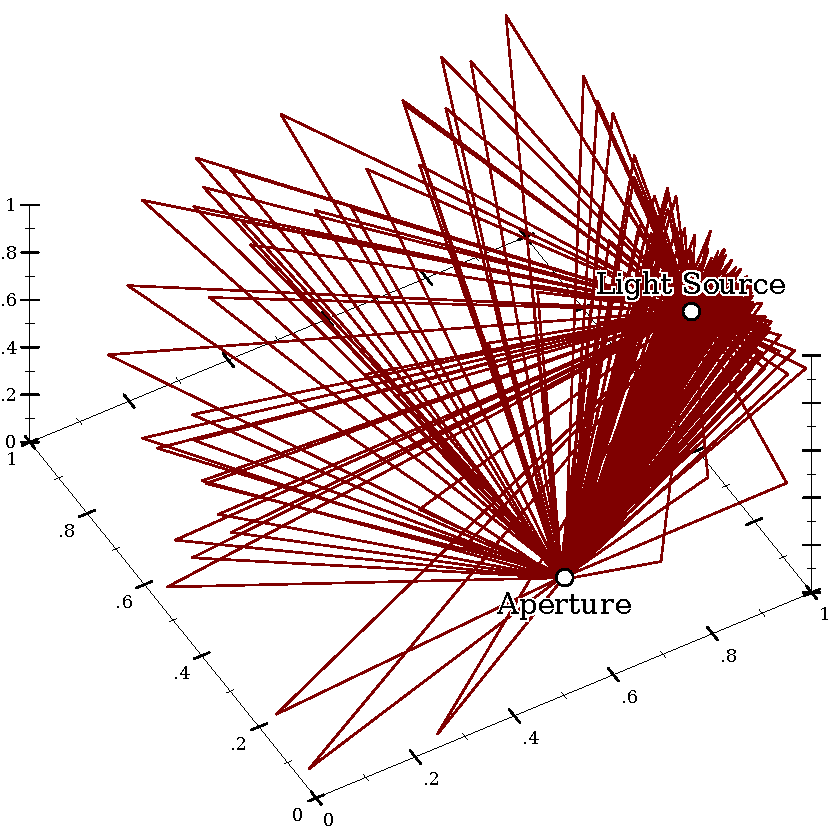
\includegraphics[width=\textwidth]{ray-tracing}
\end{minipage}
\label{fig:ray-tracing-paths}
}
\tab\tab
\subfloat[1,000,000 random paths that pass through the aperture, projected onto a plane and accumulated.]{
\begin{minipage}{0.43\textwidth}
\centering
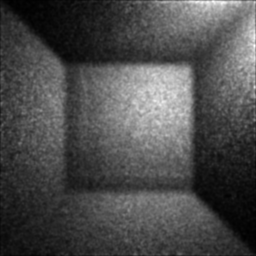
\includegraphics[width=\textwidth]{ray-tracing-projection}
\end{minipage}
\label{fig:ray-tracing-projection}
}

\subfloat[Part of the ray tracer implementation. Sampling involves computing approximate preimages under functions like this.]{
\usebox{\codebox}
\label{fig:ray-plane-intersect}
}
\caption[ ]{Stochastic ray tracing in Dr. Bayes is little more than physics simulation.}
\label{fig:ray-tracing}
\end{figure*}

\figref{fig:ray-tracing} shows the result of using Dr. Bayes for stochastic ray tracing~\cite{cit:veach-1997siggraph-mlt}.
In this instance, photons are cast from a light source in a uniformly random direction and are reflected by the walls of a square room, generating paths.
The objective is to sample, with the correct distribution, only those paths that pass through an aperture.
The smaller the aperture, the smaller the probability a path passes through it, and the more focused the resulting image.

All efficient implementations of stochastic ray tracing to date use sophisticated, specialized sampling methods that bear little resemblance to the physical processes they simulate.
The proof-of-concept ray tracer, written in Dr. Bayes, is little more than a simple physics simulation and a conditional query.


%%%%%%%%%%%%%%%%%%%%%%%%%%%%%%%%%%%%%%%%%%%%%%%%%%%%%%%%%%%%%%%%%%%%%%%%%%%%%%%%%%%%%%%%%%%%%%%%%%%%%
%%%%%%%%%%%%%%%%%%%%%%%%%%%%%%%%%%%%%%%%%%%%%%%%%%%%%%%%%%%%%%%%%%%%%%%%%%%%%%%%%%%%%%%%%%%%%%%%%%%%%
%%%%%%%%%%%%%%%%%%%%%%%%%%%%%%%%%%%%%%%%%%%%%%%%%%%%%%%%%%%%%%%%%%%%%%%%%%%%%%%%%%%%%%%%%%%%%%%%%%%%%

\section{Related Work}

\begin{comment}
Any programming language research described by the words ``bijective'' or ``reversible'' might seem to have much in common with ours.
Unfortunately, when we look more closely, we can usually draw only loose analogies and perhaps inspiration.
An example is lenses~\cite{cit:hofmann-2012popl-edit-lenses}, which are transformations from $X$ to $Y$ that can be run forward and backward, in a way that maintains some relationship between $X$ and $Y$.
Usually, a destructive, external process is assumed, so that, for example, a change from $y \in Y$ to $y' \in Y$ induces a corresponding change from $x \in X$ to some $x' \in X$.
When transformations lose information, lenses must satisfy certain behavioral laws.
In our work, no input or output is updated, and preimages are always definable regardless of non-injectivity.

Many multi-paradigm languages~\cite{cit:hanus-2007lp-multi-paradigm}, especially constraint functional languages, bear a strong resemblance to our work.
In fact, it is easy to add a $fail$ expression to our semantics, or to transform constraints into boolean program outputs.
The most obvious difference is evaluation strategy.
The most important difference is that our interpretation of programs returns \emph{distributions} of constrained outputs, rather than arbitrary single values that meet constraints.
\end{comment}

%Computing a preimage also computes an overapproximation of a subdomain's image, which generalizes interval arithmetic~\cite{cit:kearfott-1996eb-interval} to all first-order algebraic types.
%Related to this,
Our approximating semantics can be regarded as an abstract interpretation~\cite{cit:cousot-1977popl-abstract-interpretation}.
It is typical in some ways: it is sound, the abstract domain is a lattice, and the concrete (i.e. exact) semantics performs infinite computations.
It is atypical in other ways: it is used to run programs, there is no Kleene iteration, abstraction boundaries are $if$ expressions in (conceptually) infinite programs, and infinite computations are confined to a combinator library.
This last property makes our work similar to monadic abstract interpretation~\cite{cit:sergey-2013pldi-monadic-abstract}, but \lzfclang allows concrete combinators to perform uncountably many operations.

Probabilistic languages can be approximately placed into two groups: those defined by an implementation, and those defined by a semantics.

Some languages defined by an implementation are probabilistic Scheme~\cite{cit:koller-1997aaai-bayes-programs-short}, BUGS~\cite{cit:winbugs-language-short}, BLOG~\cite{cit:blog-language-short}, BLAISE~\cite{cit:blaise-language}, Church~\cite{cit:church-language-short}, and Kiselyov's embedded language for O'Caml~\cite{cit:kiselyov-2008uai-monolingual}.
The reports on these languages generally describe interpreters, compilers, and algorithms for sampling with probabilistic conditions.
Recently, Wingate et al~\cite{cit:wingate-2011nips-nonstandard} have defined the semantics of nonstandard interpretations that enable efficient inference, but do not define the languages.

Early work in probabilistic language semantics is not motivated by Bayesian concerns, and thus does not address conditioning.
Examples are Kozen~\cite{cit:kozen-1979fcs-prob-programs-short}, Hurd~\cite{cit:hurd-2002thesis}, Jones~\cite{cit:jones-1990thesis}, Ramsey and Pfeffer~\cite{cit:ramsey-2002popl-stochastic-short}, and Park~\cite{cit:park-2008toplas-prob}.
Recent semantics work tackles conditioning, such as IBAL~\cite{cit:pfeffer-2007chapter-ibal} and Fun~\cite{cit:borgstrom-2011esop-measure-transformer}.
While Fun's measure-theoretic semantics looks promising, its implementations are based on probability densities, so they cannot handle recursion or aribtrary conditions.

%%%%%%%%%%%%%%%%%%%%%%%%%%%%%%%%%%%%%%%%%%%%%%%%%%%%%%%%%%%%%%%%%%%%%%%%%%%%%%%%%%%%%%%%%%%%%%%%%%%%%
%%%%%%%%%%%%%%%%%%%%%%%%%%%%%%%%%%%%%%%%%%%%%%%%%%%%%%%%%%%%%%%%%%%%%%%%%%%%%%%%%%%%%%%%%%%%%%%%%%%%%
%%%%%%%%%%%%%%%%%%%%%%%%%%%%%%%%%%%%%%%%%%%%%%%%%%%%%%%%%%%%%%%%%%%%%%%%%%%%%%%%%%%%%%%%%%%%%%%%%%%%%

\section{Conclusions and Future Work}

To allow recursion and arbitrary conditions in probabilitic programs, we combined the power of measure theory with the unifying elegance of arrows. We
\begin{enumerate}
	\item Defined a transformation from first-order programs to arbitrary arrows.
	\item Defined the bottom arrow as a standard translation target.
	\item Derived the uncomputable preimage arrow as an alternative target.
	\item Derived a sound, computable approximation of the preimage arrow, and enough computable lifts to transform programs.
\end{enumerate}
Critically, the preimage arrow's lift from the bottom arrow distributes over bottom arrow computations.
Our semantics thus generalizes this process to all programs: 1) encode a program as a bottom arrow computation; 2) lift this computation to get an uncomputable function that computes preimages; 3) distribute the lift; and 4) replace uncomputable expressions with sound approximations.

Our semantics trades efficiency for simplicity by threading a constant, tree-shaped random source (Section~\ref{sec:threading-and-indexing}).
Passing subtrees instead would make $random$ a constant-time primitive, and allow combinators to detect lack of change and return cached values.
Other future optimization work includes creating new sampling algorithms, and using other easily measured but more expressive set representations, such as parallelotopes~\cite{cit:amato-2012tcs-parallelotopes}.
On the theory side, we intend to explore preimage computation's connection to type checking and type inference, investigate ways to integrate and leverage polymorphic type systems, and find the conditions under which preimage refinement is complete in the limit.

More broadly, we hope to advance Bayesian practice by providing a rich modeling language with an efficient, correct implementation, which allows general recursion and any computable, probabilistic condition.

%%%%%%%%%%%%%%%%%%%%%%%%%%%%%%%%%%%%%%%%%%%%%%%%%%%%%%%%%%%%%%%%%%%%%%%%%%%%%%%%%%%%%%%%%%%%%%%%%%%%%
%%%%%%%%%%%%%%%%%%%%%%%%%%%%%%%%%%%%%%%%%%%%%%%%%%%%%%%%%%%%%%%%%%%%%%%%%%%%%%%%%%%%%%%%%%%%%%%%%%%%%
%%%%%%%%%%%%%%%%%%%%%%%%%%%%%%%%%%%%%%%%%%%%%%%%%%%%%%%%%%%%%%%%%%%%%%%%%%%%%%%%%%%%%%%%%%%%%%%%%%%%%



%\appendix
%\section{Appendix Title}
%This is the text of the appendix, if you need one.

%\acks
%Acknowledgments, if needed.

\mathversion{normal}

\bibliographystyle{splncs03}
\bibliography{local-cites}

\end{document}
